\section{Experimental Results}
\label{sec:experiments}

We compare ExtRA with 
multiple strong baselines on extracting aspect terms from user reviews. 
We first introduce the dataset and the competing models, then
show the quantitative evaluation as well as qualitative analysis for
different models.

\subsection{Dataset}
\label{sec:dataset}
We use the customer review corpora of 6 kinds of product and service
\footnote{The data is available from
	\url{http://times.cs.uiuc.edu/~wang296/Data/} and 
	\url{https://www.yelp.com/dataset}} collected from popular websites, 
including Amazon, TripAdvisor and Yelp. 
The number of hotel reviews \cite{Wang2011LearningOD} in the original
corpus is huge. 
Therefore, we randomly sample 20\% of the reviews to perform our experiments.
The statistics of the corpora are shown in~\tabref{table:dataset}.

\begin{table}[th!]
	\small
	\centering
	\vspace{-0.3cm}
	\caption{Dataset statistics.} 
	\label{table:dataset}
	\vspace{-0.2cm}
	\begin{tabular}{|c|c|r|}
		\hline
		\textbf{Product type} & \textbf{Source} & \textbf{\#Reviews} \\ \hline \hline
		hotel        & TripAdvisor & 3,155,765   \\\hline
		mobile phone & Amazon & 185,980  \\\hline
		mp3 player   & Amazon & 30,996   \\\hline
		laptop       & Amazon & 40,744   \\\hline
		cameras & Amazon & 471,113  \\\hline
		restaurant   & Yelp & 269,000   \\\hline
	\end{tabular}
	\vspace{-0.2cm}
\end{table}

%\label{sec:evaldataset}
Existing published aspect extraction datasets ~\cite{hu2004mining,popescu2007extracting,pavlopoulos2014aspect,ding2008holistic} 
include only fine-grained aspects from reviews,
which are not suitable for evaluating the performance of 
prominent aspects extraction. 
Therefore, we build a new evaluation dataset particularly 
for this task.
%\KZ{We need to explain why the data set is for 5 aspect only, not 10, 15?}
Following the previous work 
%Ganu et al
~\cite{ganu2009beyond,brody2010unsupervised,zhao2010jointly,wang2015sentiment} as well as
the popular commercial websites (e.g. TripAdvisor), 
which commonly label 4 to 9 prominent aspects for
rating, we respectively set $K$ as $5$, $7$ and $9$
in the following experiments.
We have five annotators in total.
We ask each annotator who are familiar with the domain 
to give $K$ aspect terms which they think are most important
for each category. 
%In total, there are 25 aspect terms
%for each product type (including duplicates).
%Our annotated ground truths are all words by design, 
%since our baseline models can only extract aspect words.
%For example, the one set of annotations for hotel is 
%{\em room, price, location, service, utility}, and the annotations
%for restaurant is
%{\em location, price, food, service, cleanness}. 
\footnote{The 
	complete labeled set of ExtRA are released at \url{https://drive.google.com/file/d/10t0Y4YSUtW7cRQWgfaHvLvECjOaPRuWo/view?usp=sharing}.
}

One prominent aspect could be expressed by different terms.
Thus, it is difficult to achieve a satisfied inner-agreement.
We propose two evaluation methods, especially the 
soft accuracy in \secref{sec:quaneval} to compensate this problem.
To acquire a relatively higher inner-agreement, 
we educate the annotators with top 100 frequent aspect candidates
as hints. Though, they are not required to pick up labels from 
the candidates.
The inter-annotator agreement of each
product type shown in \tabref{tab:agreement} is computed as the average jaccard similarity between every two annotators.
As can be seen, for the category \textit{hotel},
the agreement between annotators 
achieves the highest value $0.44$ when $K$ is $5$,
which means that $K=5$ is the most reasonable 
number of prominent aspects for \textit{hotel}.
Similarly, $K=9$ is the most appropriate value for
\textit{mp3}, \textit{cameras}, \textit{mobile phone} and \textit{laptop}.
and it is better to set $K$ as $7$ for \textit{restaurant}.
As seen from the released evaluation dataset,
although the jaccard agreements on \textit{cameras}
and \textit{laptop} is relatively low,
the collected labels are still highly correlated on semantics.

\begin{table}[!h]
	\small
	\centering
%		\vspace{-0.3cm}
	\caption{Inner-annotator agreements}
	\label{tab:agreement}
%	\begin{tabular}{|p{2.5cm}<{\centering}|c|c|c|c|c|c|}
	\begin{tabular}{|c|c|c|c|c|c|c|}
		\hline
		\diagbox[width=9em]{Agreement}{Category} & hotel & mp3 & cameras & \begin{tabular}[c]{@{}l@{}}mobile\\ phone\end{tabular} & laptop & restaurant \\\hline\hline
		$K=5$    & {\bf 0.440}  & 0.258 & 0.201    & 0.148     & 0.131   & 0.464          \\\hline
		$K=7$    & 0.362  & 0.375 & 0.277  & 0.319  & 0.225  & {\bf 0.497}        \\\hline
		$K=9$    & 0.365  & {\bf 0.405} & {\bf 0.301}    & {\bf 0.431}   &  {\bf 0.250}  & 0.456         \\\hline
	\end{tabular}
\end{table}


%\begin{table}[th]
%	\small
%	\centering
%	\caption{Selected ground-truth labels.}
%	\label{table:labels}
%	\begin{tabular}{|c|l|}
%		\hline
%	Product type & Prominent aspects \\ \hline\hline
%		hotel
%		%			& price location room service bath staff \\\hline 
%		& room price location service utility \\ \hline
%		
%		camera
%		%			& battery image lens price appearance storage focus design mode memory carry operation \\\hline
%		& image lens battery memory carry \\ \hline
%		
%		restaurant
%		%			& food price location service environment cleans \\\hline
%		& location price food service cleanness \\ \hline
%	\end{tabular}
%\end{table}


%We aim to extract $K$ prominent aspects from review texts
%which are most important and representative
%for the given kind of products or services. 

\subsection{Baselines and ExtRA}
\label{sec:base}
We introduce three topic modeling based baselines for the task.
These are \textbf{LDA}~\cite{Blei2003LatentDA}, 
\textbf{BTM}~\cite{DBLP:journals/tkde/ChengYLG14} and  
\textbf{MG-LDA}~\cite{titov2008modeling}. MG-LDA is a strong
baseline which attempts to capture multi-grain topics (i.e. global \& local), where the local topics correspond to the rateable prominent aspects.
We treat each review as a document and perform those models
to extract $K$ topics.
% Each topic is expected to model an 
%prominent aspect for the given product or service.
Then, we select most probable words in 
each topic as our extracted aspect terms. 
To prevent extracting the same aspects ($w$) from different topics, 
we only keep $w$ for the topic $t$ with the highest 
probability $p(w|t)$ value, then re-select aspects for the other 
topics until we get $K$ different aspects. 
For fair comparison among different models, the number of 
target aspects $K$ is set as $5$, $7$ and $9$ separately. 
The hyper-parameter of 
MG-LDA (global topics) is set to 30 with fine-tuning.

Another syntactic rule-based baseline model 
\textbf{RuleExt} is from the first step of 
the proposed method. 
After extracting the aspect candidates using
\emph{rules} (i.e. Rule 1$\sim$ 3) and \emph{extension rules}
(i.e. Rule E1$\sim$ E3) in \secref{sec:candidate}, 
we sort the aspect candidates by 
their counts of extracted occurrences. 
Then select the top $K$ 
candidates as the prominent aspects.

\textbf{ABAE}~\cite{DBLP:conf/acl/HeLND17}  is a neural based model that can
to infer $K$ aspect types. 
Each \emph{aspect type} is a ranked list of representative words.
To generate $K$ prominent aspects, 
we first infer $K$ aspect types using \emph{ABAE}, 
then select the most representative word from each
aspect type. We set the number of training
epochs as $100$ using the code \footnote{https://github.com/ruidan/Unsupervised-Aspect-Extraction} released by author.

Note that the top aspect terms from the baseline methods, 
inevitably contain some sentiment words and opinions, like \textit{
excellent, nice, great, etc}. 
To remedy this, we post process the results for baselines methods
in order to reverse the nouns only.
%We evaluate our framework as well as 
%the above baselines on the evaluation dataset.

%\paragraph{ExtRA Settings}
%\label{ourmodels}

For \textbf{ExtRA},  
we use WordNet $3.0$ and the Probase snapshot
released in $2012$
which consists of $69,707,026$
distinct concept-instance pairs in total.
We use GloVe embeddings 
with 300 dimensions, trained from 840B tokens using common crawl data. 
As described in \secref{sec:clusters},
we use silhouette score to automatically tune the 
cluster number $Z$ when generating the
final prominent aspect clusters for $co_i^{(j)}$ by
K-means.
We search the value of $Z$ from $1$ to $min(V-2, \frac{V}{2})$,
where $V=|co_i^{(j)}|$.
The optimal $Z$ achieves the 
highest silhouette score after clustering.

%The comparison of quantitative results are shown in \tabref{table:comparison}.}

\subsection{Evaluation}
\label{sec:endeval}
In this section, we compare ExtRA with five baseline models 
both quantitatively and qualitatively.

\subsubsection{Quantitative Evaluation}
\label{sec:quaneval}


%First, we perform two experiments to justify our aspect taxonomy construction stage:
%\begin{figure}[h]
%	\centering
%	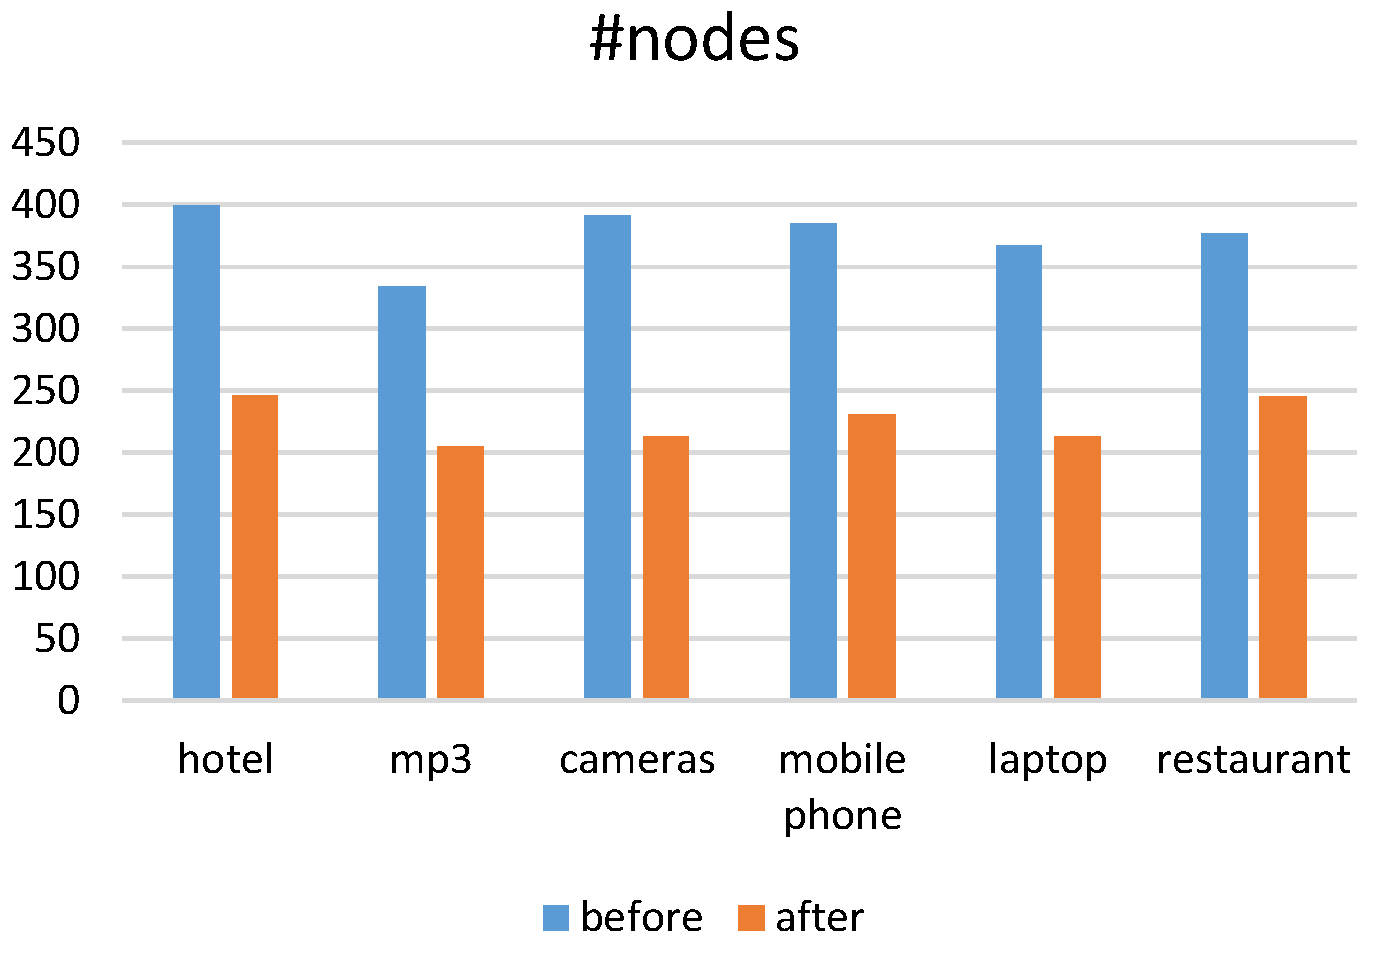
\includegraphics[width=0.48\columnwidth]{figures/1.pdf}
%	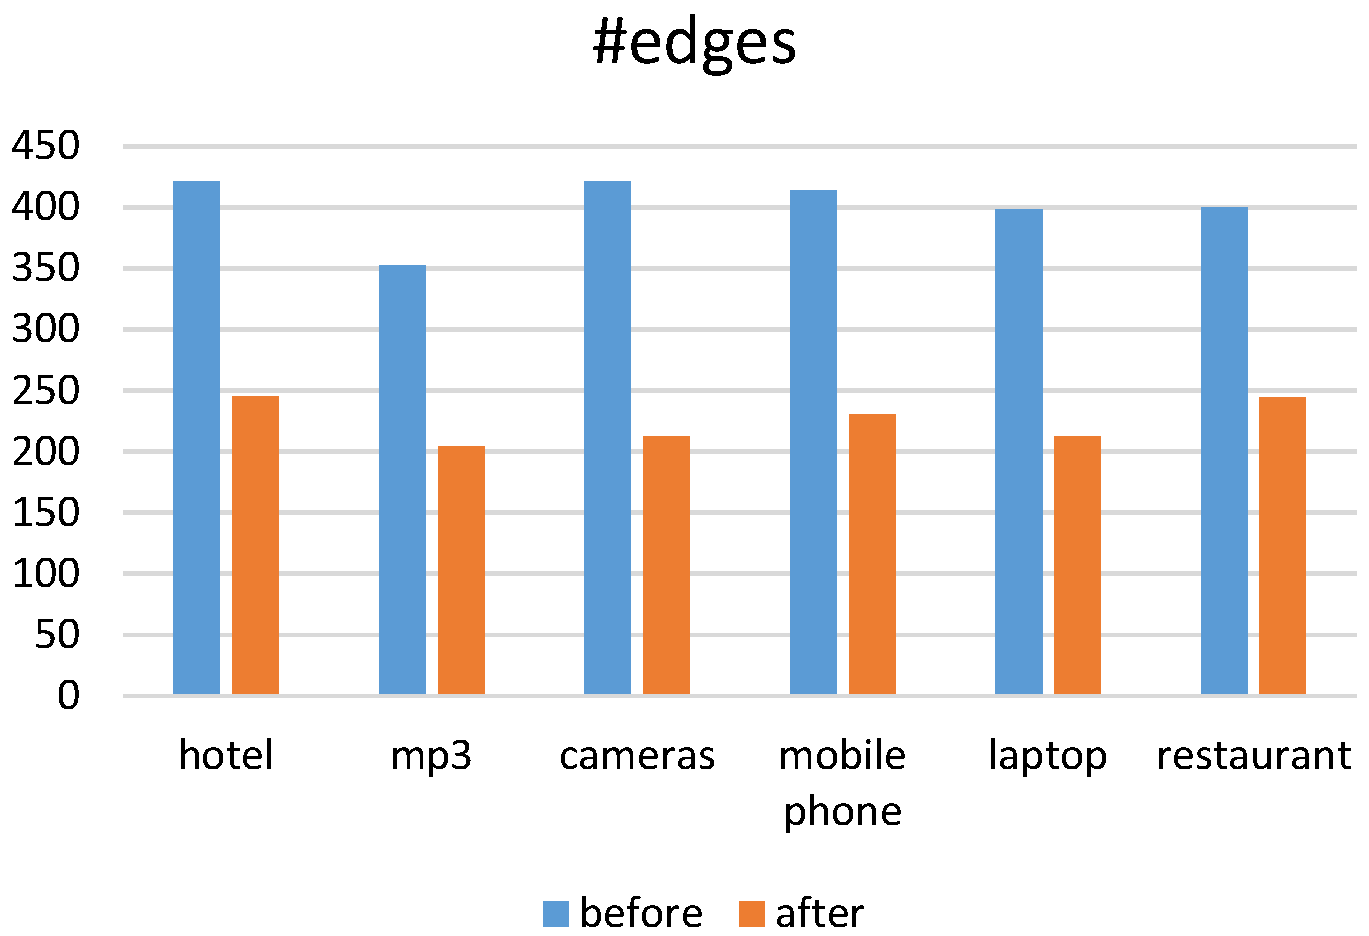
\includegraphics[width=0.48\columnwidth]{figures/2.pdf}
%	\caption{Statistics of induced aspect taxonomy before and after taxonomy minimization}
%	\label{fig:size}
%	\vspace{-10pt}
%\end{figure}

We evaluate our model as well as above baselines on the evaluation dataset described above.
We have $H=5$ human annotators in total.
We did not remove the duplicate aspect labels for the qualitative evaluation, 
since the repeated aspects are assume to be better.

\begin{table}[!th]
	\small
	\centering
	\caption{Comparison of \emph{hard} (upper row) \& \emph{soft} (lower row) accuracies using different models with optimal $K$ for each category.}
	\label{table:comparison}
	\begin{tabular}{|c|c|c|c|c|c|c|}
		\hline
		&    LDA  & BTM &  \begin{tabular}[c]
			{@{}l@{}}MG-\\LDA \end{tabular}  & ABAE & RuleExt & ExtRA \\ \hline \hline
		\multirow{2}{*}{\begin{tabular}{cc}hotel\\($K=5$)\end{tabular}} & 0.360 & 0.360 & 0.360  &  0.120  & 0.520 & \textbf{0.560} \\ \cline{2-7}
		&  0.613 & 0.625 & 0.614 & 0.394  & 0.704  &  \textbf{0.769} \\ \hline
		\multirow{2}{*}{\begin{tabular}{cc}mp3\\($K=9$)\end{tabular}}  & 0.089 & 0.089 & 0.178  & 0.000 & 0.222 & \textbf{0.467} \\ \cline{2-7} 
		&   0.396 & 0.402 & 0.542 & 0.304 & 0.547 &  \textbf{0.689} \\ \hline
		\multirow{2}{*}{\begin{tabular}{cc}cameras\\($K=9$)\end{tabular}}  & 0.178 & 0.133 & 0.133 & 0.133 & 0.133  &  \textbf{0.422} \\ \cline{2-7} 
		&   0.509 & 0.485 & 0.490 & 0.441 & 0.507  & \textbf{0.678} \\ \hline
		\multirow{2}{*}{\begin{tabular}{cc}mobile phone\\($K=9$) \end{tabular}}  & 0.200 & 0.200 & 0.222 & 0.000  & 0.333 & \textbf{0.511}  \\ \cline{2-7}
		&   0.488 & 0.505 & 0.524 & 0.227 & 0.633  & \textbf{0.701} \\ \hline
		\multirow{2}{*}{\begin{tabular}{cc}laptop\\($K=9$)\end{tabular}}   & 0.200 & 0.044 & 0.200 & 0.000 & 0.200  &  \textbf{0.311} \\ \cline{2-7} 
		&   0.491 & 0.364 & 0.504 & 0.261 & 0.516  &  \textbf{0.630} \\ \hline
		\multirow{2}{*}{\begin{tabular}{cc}restaurant\\($K=7$)\end{tabular}}  & 0.257 & 0.114 &0.286 & 0.000  & 0.371 & \textbf{0.600} \\ \cline{2-7} 
		&   0.548 & 0.403 & 0.560& 0.232 & 0.627  & \textbf{0.749} \\ \hline
	\end{tabular}
\end{table}

%Because there are duplicates in the label set, aspect terms that are repeated are assume to be better. 
%The labels provided by the annotators are aggregated together without removing duplicated words, so we have 25 words in total.
%This is to ensure that the information about the different importances of aspects is preserved.
%When evaluating the models, 
%we compare the 5 aspect words generated by the models with those provided 
%by the annotators. 
For a given category, we first calculate the percentage of the $H*K$ labels that exactly match one of the $K$ aspect terms generated by the model as the \textit{hard accuracy} 
%(i.e. the first line for each category in \tabref{tab:comparison}) 
of the model. 
Formally, $Aspects(m) = [a_1, a_2, ..., a_K]$ denotes 
the $K$ prominent aspects generated from model $m$ for 
the given category.
$L = [l_1, l_2, ..., l_{H*K}]$ are the $H*K$ golden aspect terms,
where $L^{(h)}= [l_{(h-1)*K+1}, ..., l_{h*K}]$ are from the $h$-th annotator.
The hard accuracy is defined as:
\begin{equation}
hacc(m) = \frac{\sum_{i=1}^{H*K}{hit(Aspects(m), l_i)}}{25}
\end{equation}

\begin{equation}
hit(Aspects(m), l_i) = 
\begin{cases}
1, & l_i \in Aspects(m) \\
0, & \text{otherwise, }
\end{cases}
\end{equation}

%We show the comparison results in \tabref{table:comparison}.
%Formally, 
%$Aspects(m, c) = [a_1, a_2, a_3, a_4, a_5]$ denotes the $5$ 
%prominent aspects generated from model $m$ given the category $c$.
%$[l_1, l_2, ..., l_{25}]$ is the 25 ground-truths annotated by
%humans. 
%We formulate the hard accuracy measure as follows:
%\begin{equation}
%hacc(m, c) = \frac{\sum_{i=1}^{25}{hit(Aspects(m, c), l_i)}}{25}
%\end{equation}
%\begin{equation}
%hit(Aspects(m, c), l_i) = 
%\begin{cases}
%1 &  \text{, if $l_i\in Aspects(m, c)$} \\
%0 &  \text{, otherwise}
%\end{cases}
%\end{equation}
%We formulate the hard accuracy measure as follows.
%$Aspects(m, c) = [a_1, a_2, a_3, a_4, a_5]$ denotes the $5$ 
%prominent aspects generated from model $m$ given the category $c$.
%$[l_1, l_2, ..., l_{25}]$ is the 25 ground-truths annotated by
%humans.

\begin{figure*}[!ht]
	\centering
	\begin{subfigure}{.333\textwidth}
		\centering
		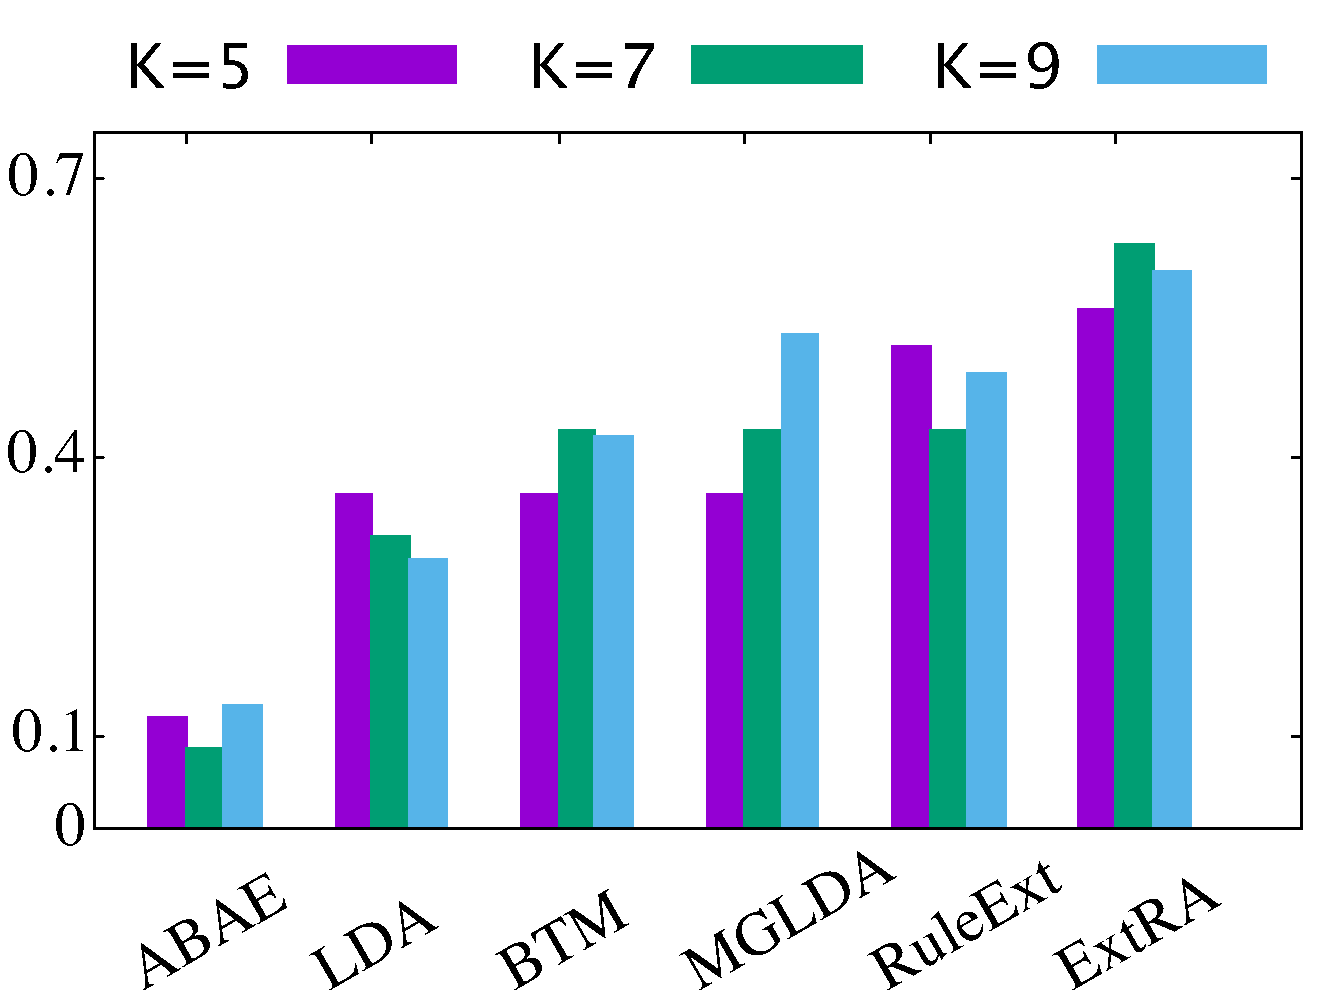
\includegraphics[width=0.99\linewidth]{figures/hotel_h}
		\caption{hotel}
		\label{fig:hotel_h}
	\end{subfigure}%
	\begin{subfigure}{.333\textwidth}
		\centering
		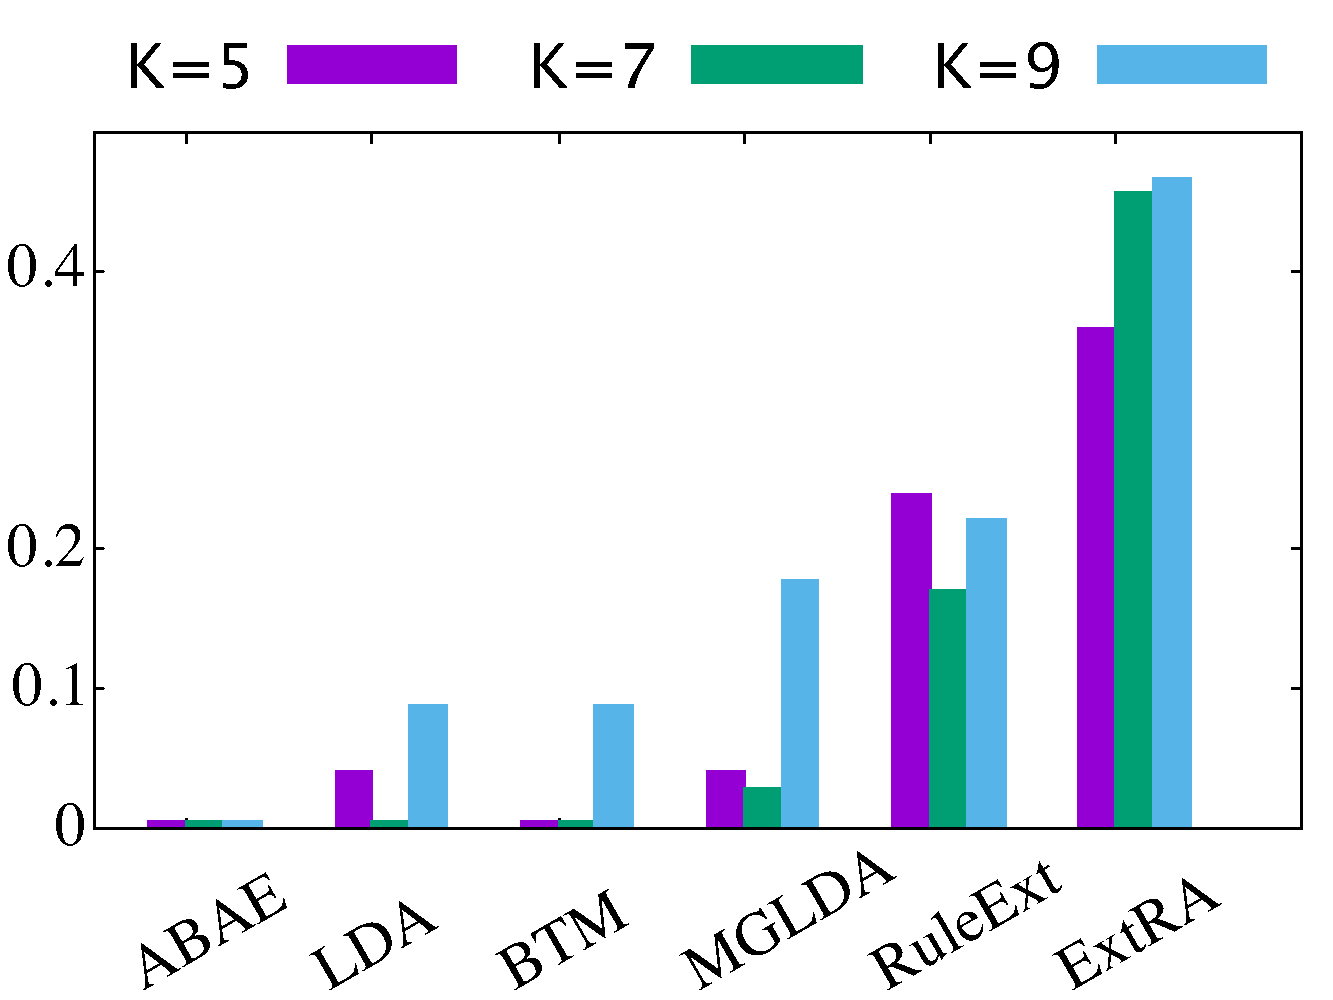
\includegraphics[width=0.99\linewidth]{figures/mp3_h}
		\caption{mp3}
		\label{fig:mp3_h}
	\end{subfigure}%
	\begin{subfigure}{.333\textwidth}
		\centering
		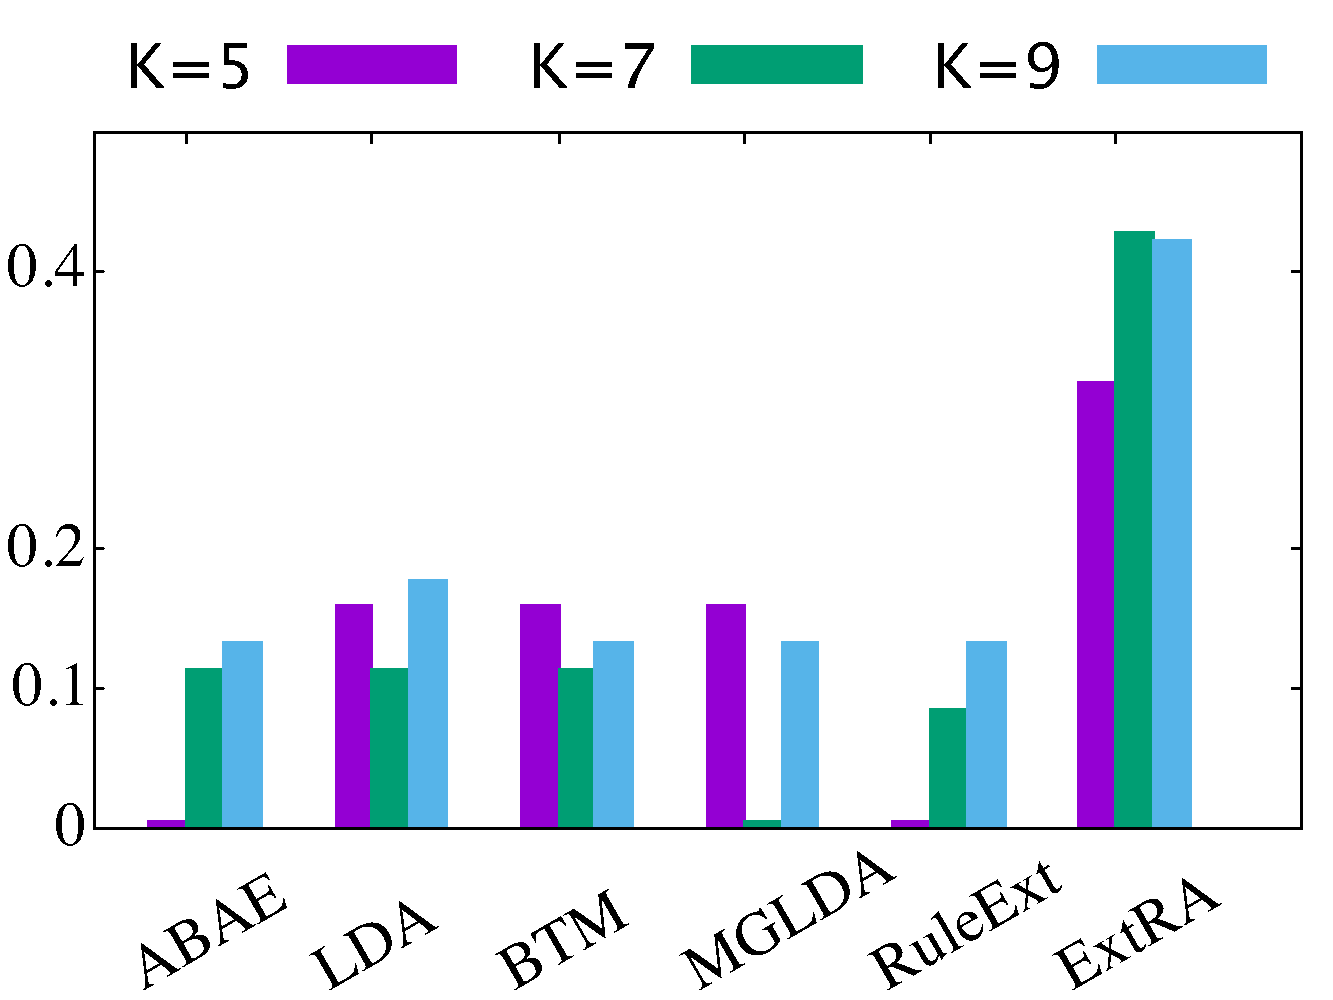
\includegraphics[width=0.99\linewidth]{figures/cameras_h}
		\caption{cameras}
		\label{fig:cameras_h}
	\end{subfigure}
	
	\begin{subfigure}{.333\textwidth}
		\centering
		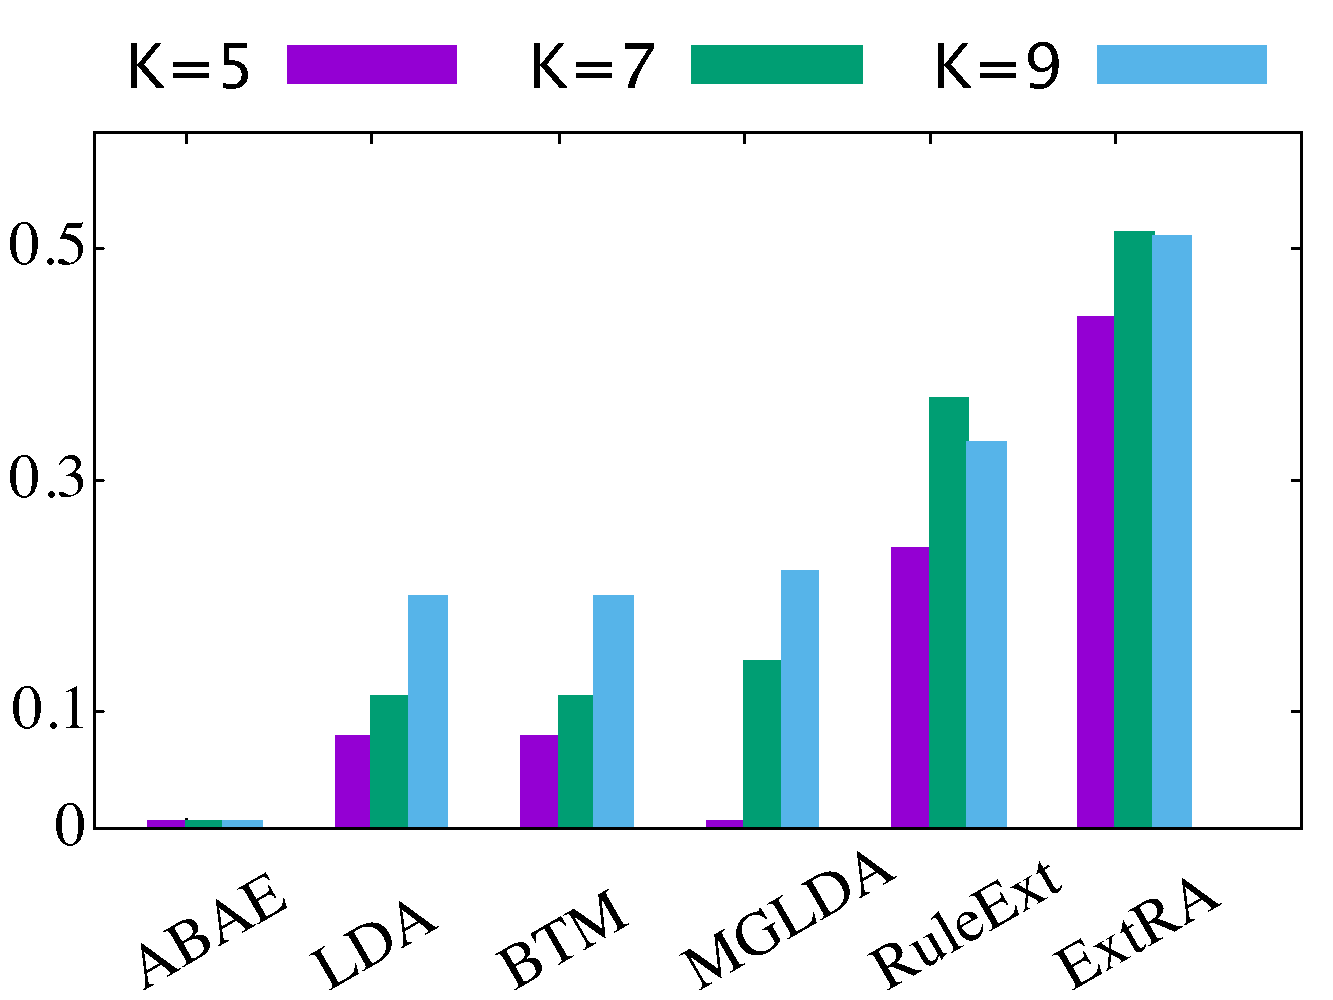
\includegraphics[width=0.99\linewidth]{figures/mobilephone_h}
		\caption{mobile phone}
		\label{fig:mobilephone_h}
	\end{subfigure}%
	\begin{subfigure}{.333\textwidth}
		\centering
		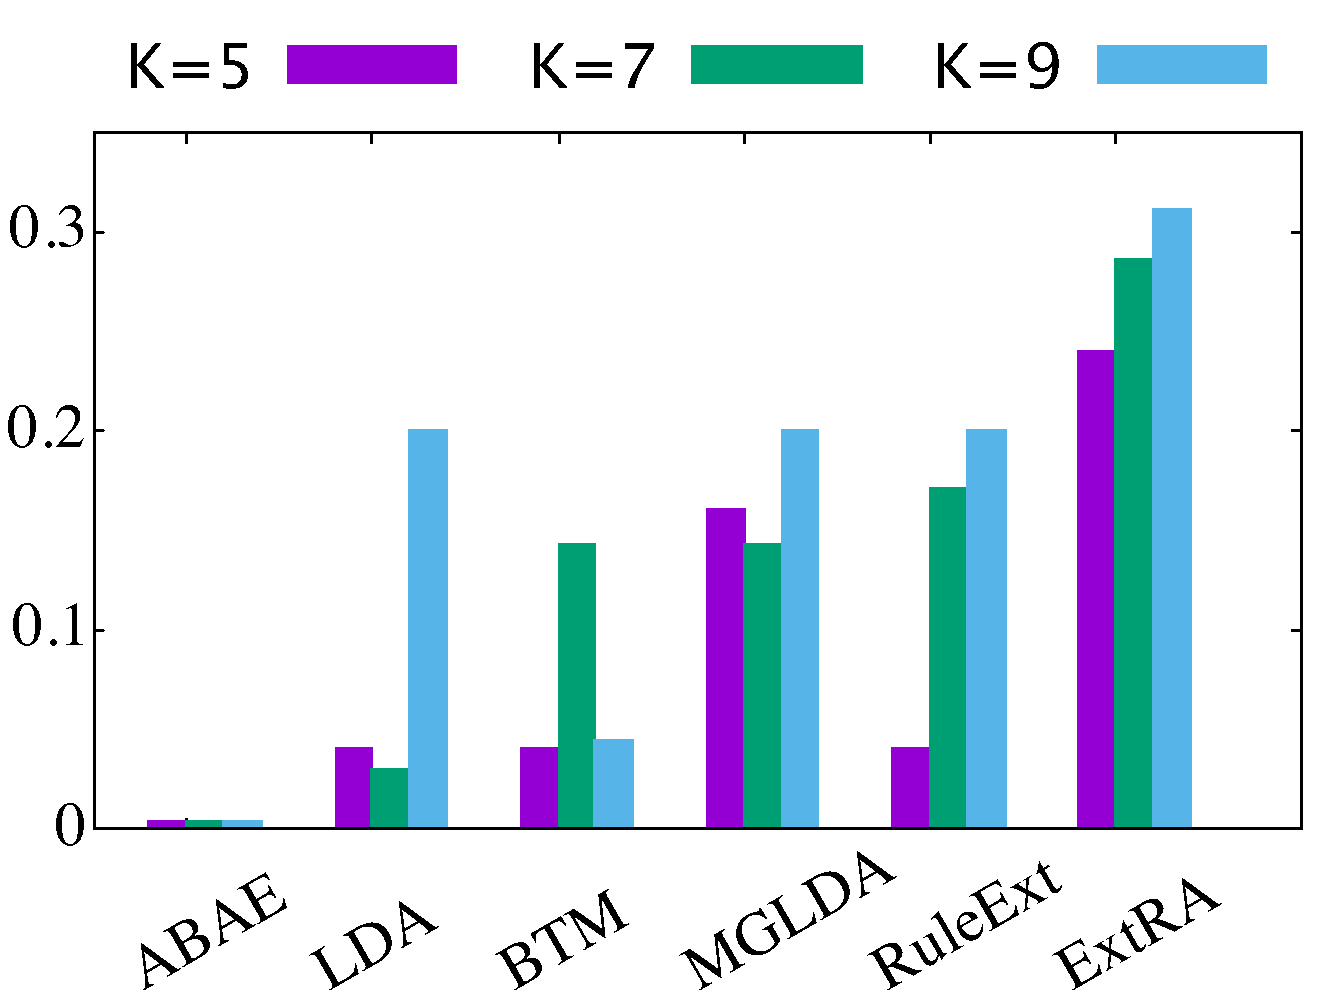
\includegraphics[width=0.99\linewidth]{figures/laptop_h}
		\caption{laptop}
		\label{fig:laptop_h}
	\end{subfigure}%
	\begin{subfigure}{.333\textwidth}
		\centering
		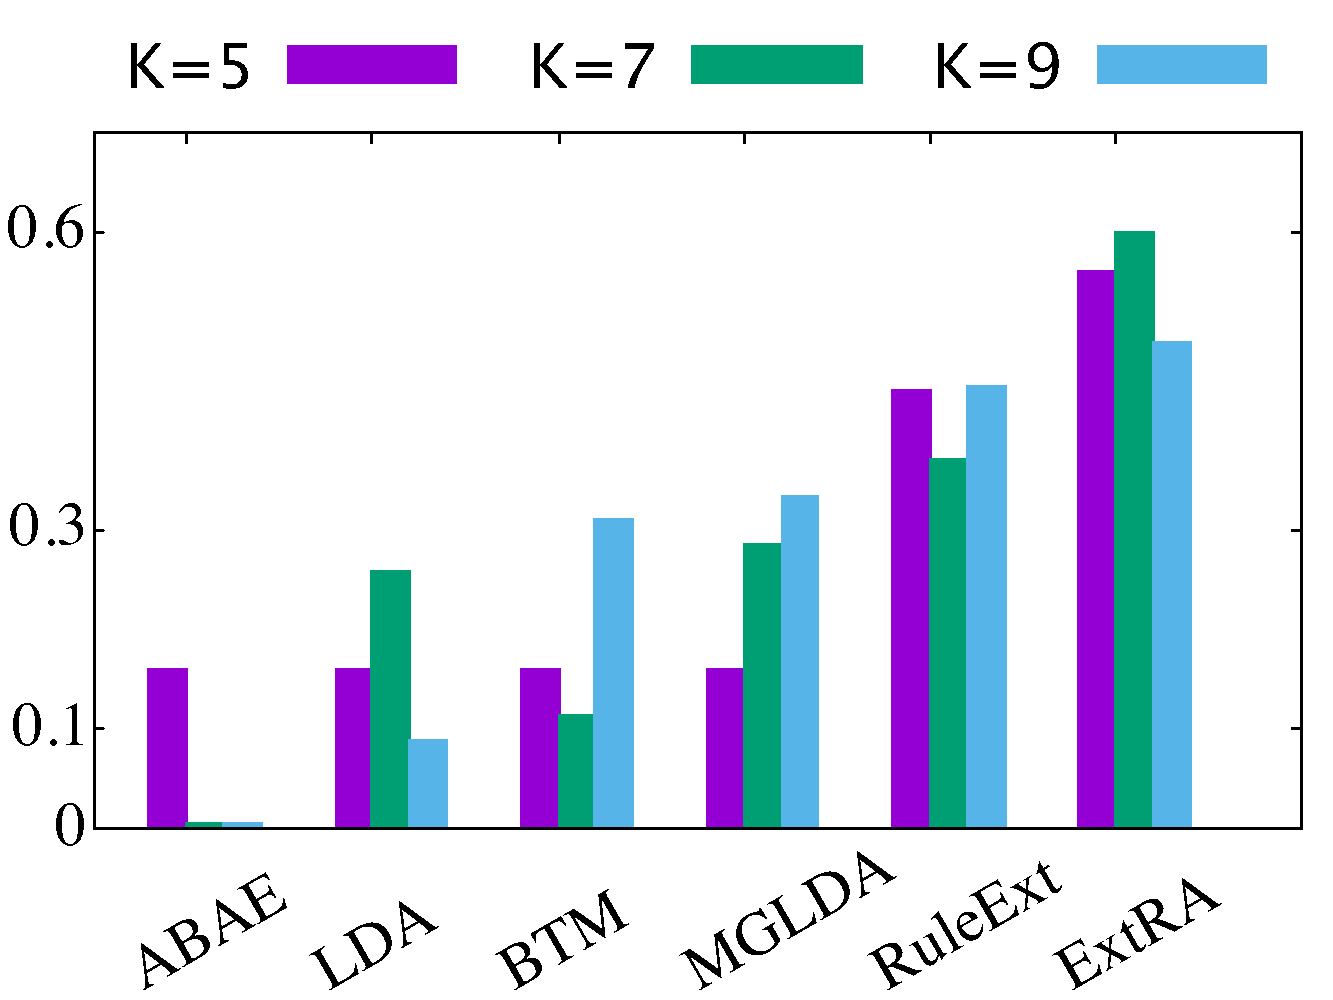
\includegraphics[width=0.99\linewidth]{figures/restaurant_h}
		\caption{restaurant}
		\label{fig:restaurant_h}
	\end{subfigure}
	
	\caption{Comparison of hard accuracies on all $K$s and categories }
	\label{fig:comparison_all_h}
\end{figure*}

However, counting the number of exact matches 
makes the accuracy score discrete and coarse. 
Besides, it penalizes aspect terms that don't match the label
but actually have similar meanings.
%To remedy this, we use the semantic similarity between
%terms as a \emph{soft accuracy}  measure which is
%computed as follows.

\begin{figure*}[!ht]
	\centering
	\begin{subfigure}{.333\textwidth}
		\centering
		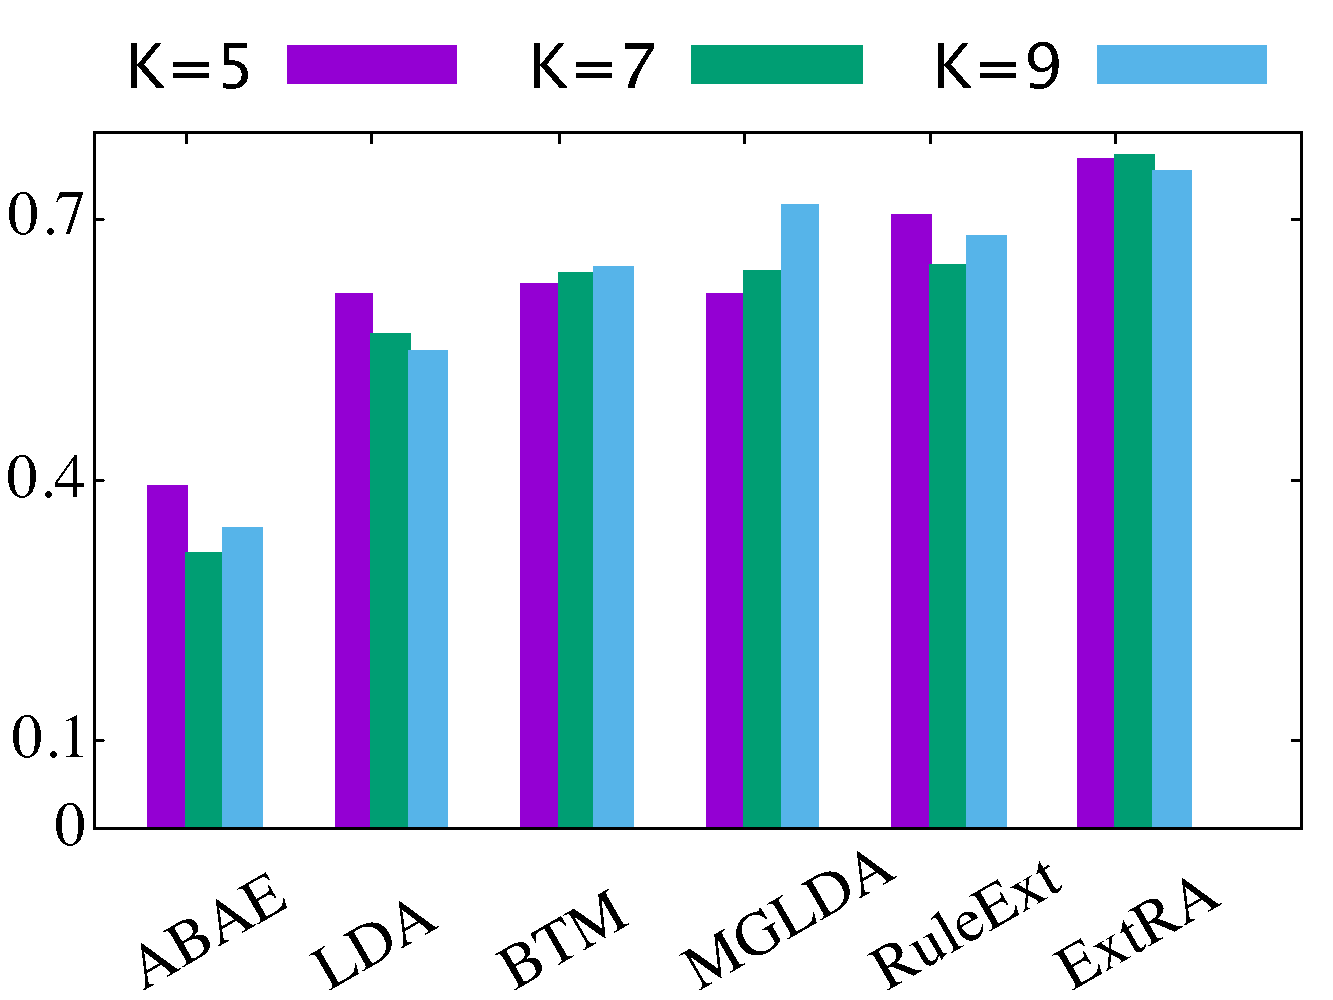
\includegraphics[width=\linewidth]{figures/hotel_s}
		\caption{hotel}
		\label{fig:hotel_s}
	\end{subfigure}%
	\begin{subfigure}{.333\textwidth}
		\centering
		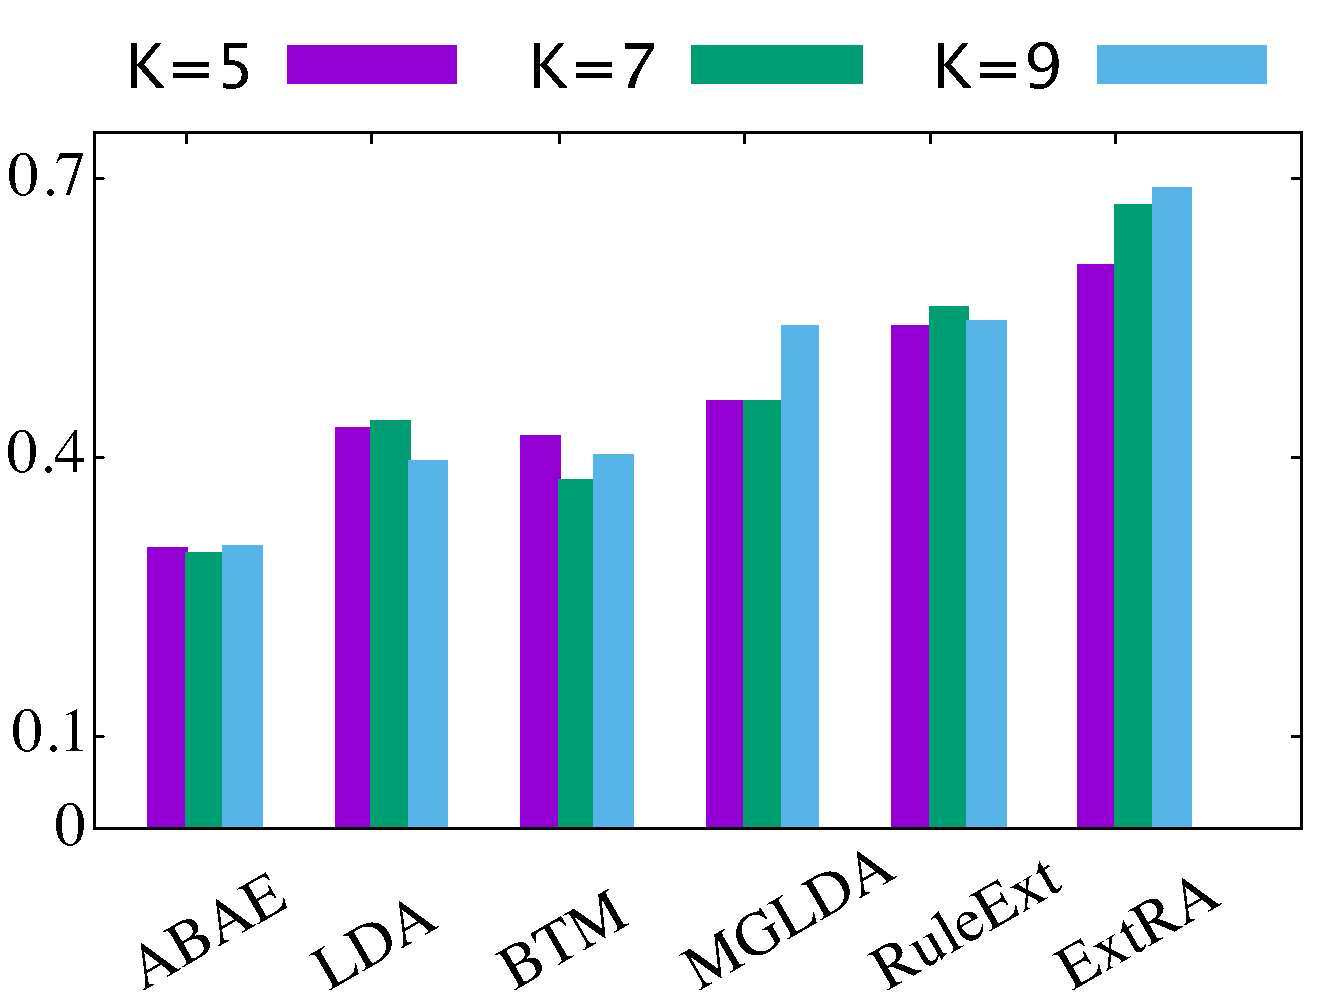
\includegraphics[width=\linewidth]{figures/mp3_s}
		\caption{mp3}
		\label{fig:mp3_s}
	\end{subfigure}%
	\begin{subfigure}{.333\textwidth}
		\centering
		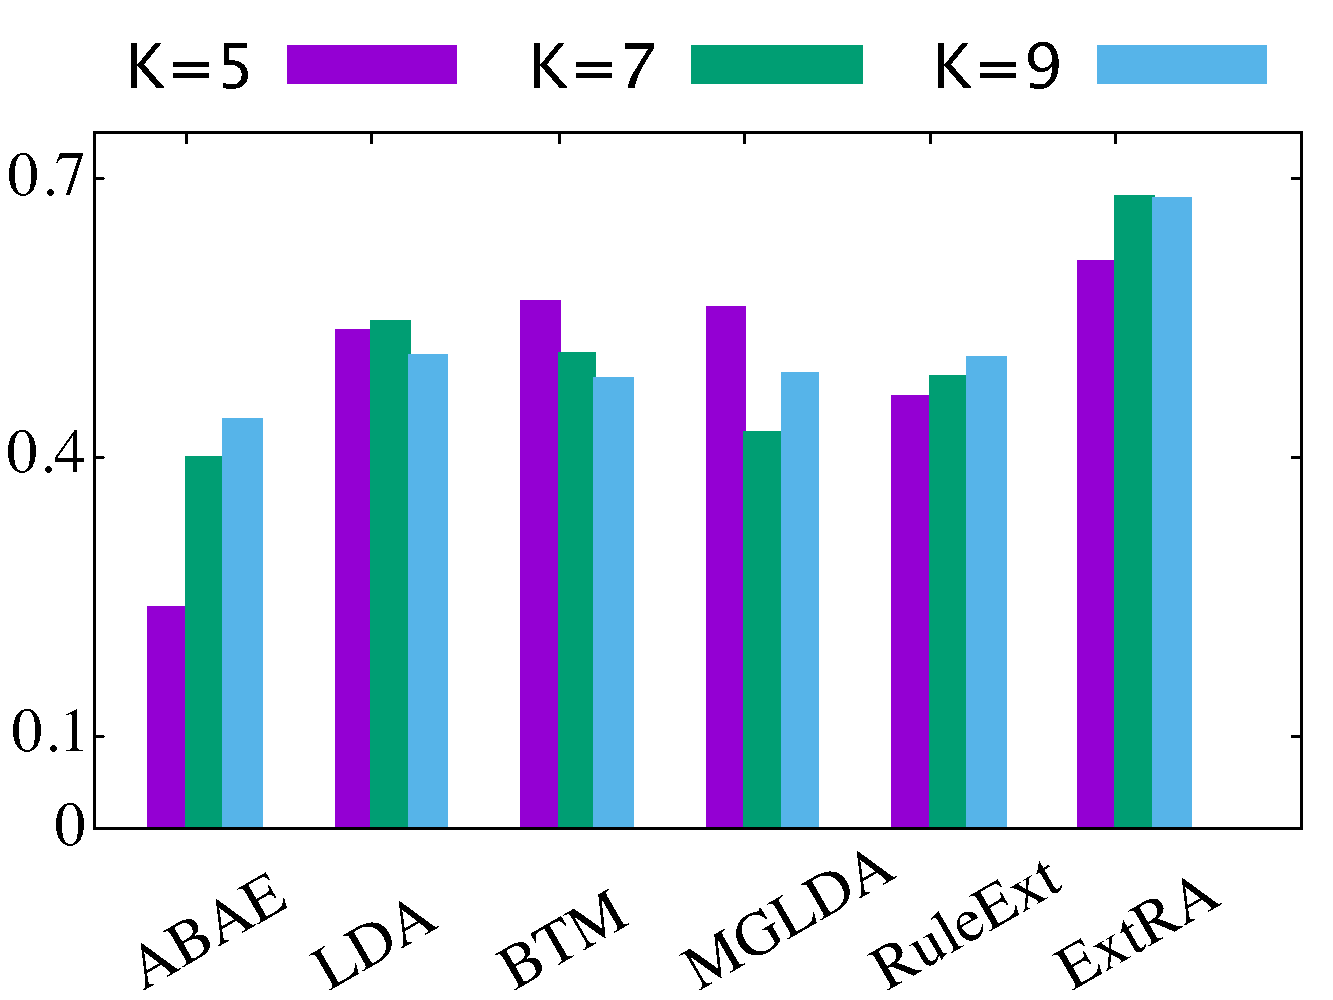
\includegraphics[width=\linewidth]{figures/cameras_s}
		\caption{cameras}
		\label{fig:cameras_s}
	\end{subfigure}
	
	\begin{subfigure}{.333\textwidth}
		\centering
		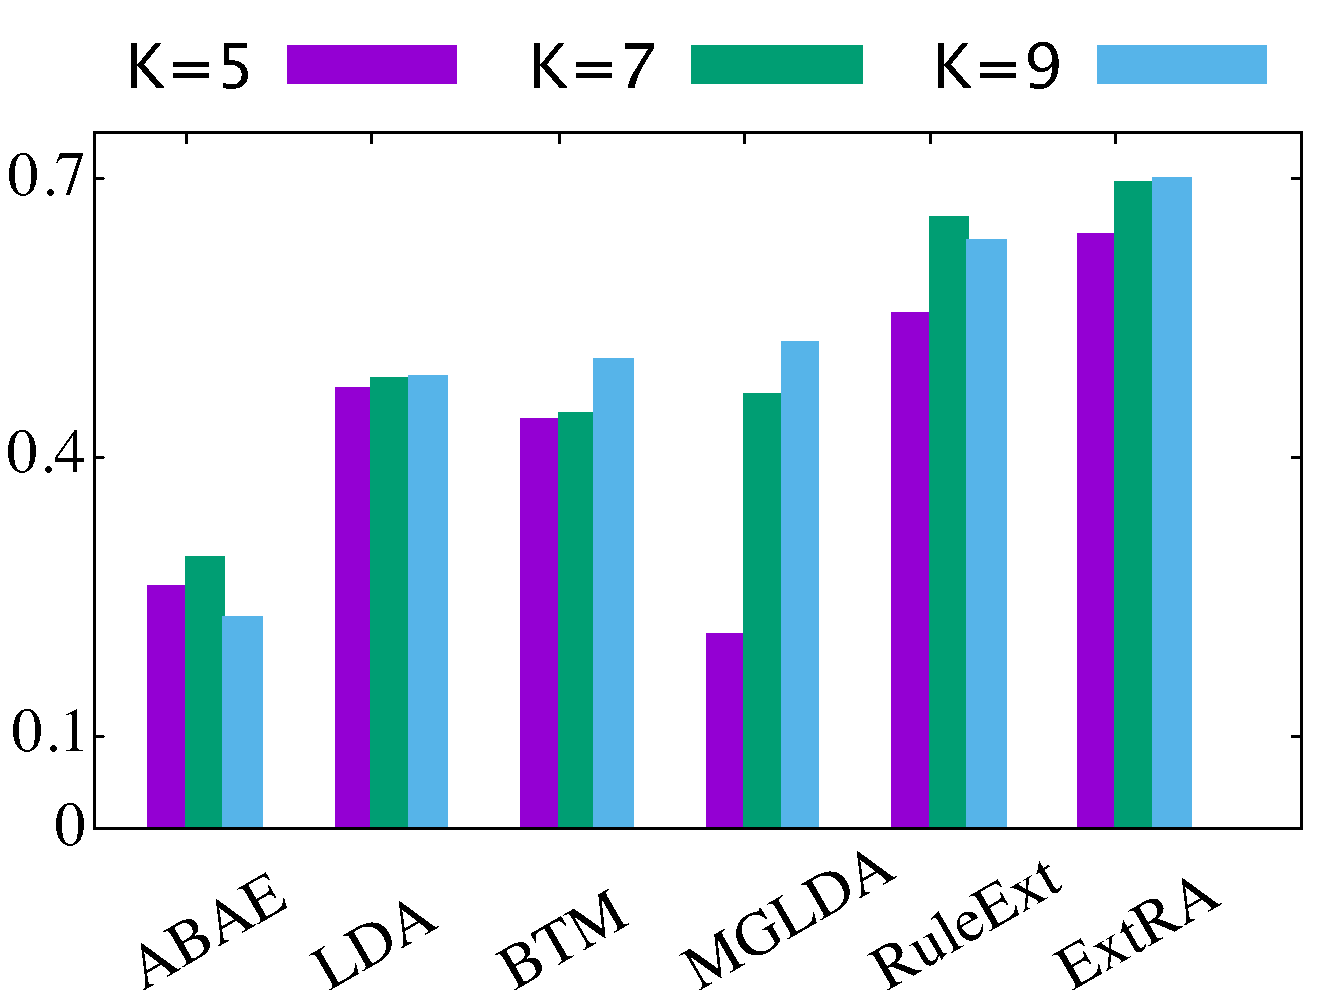
\includegraphics[width=\linewidth]{figures/mobilephone_s}
		\caption{mobile phone}
		\label{fig:mobilephone_s}
	\end{subfigure}%
	\begin{subfigure}{.333\textwidth}
		\centering
		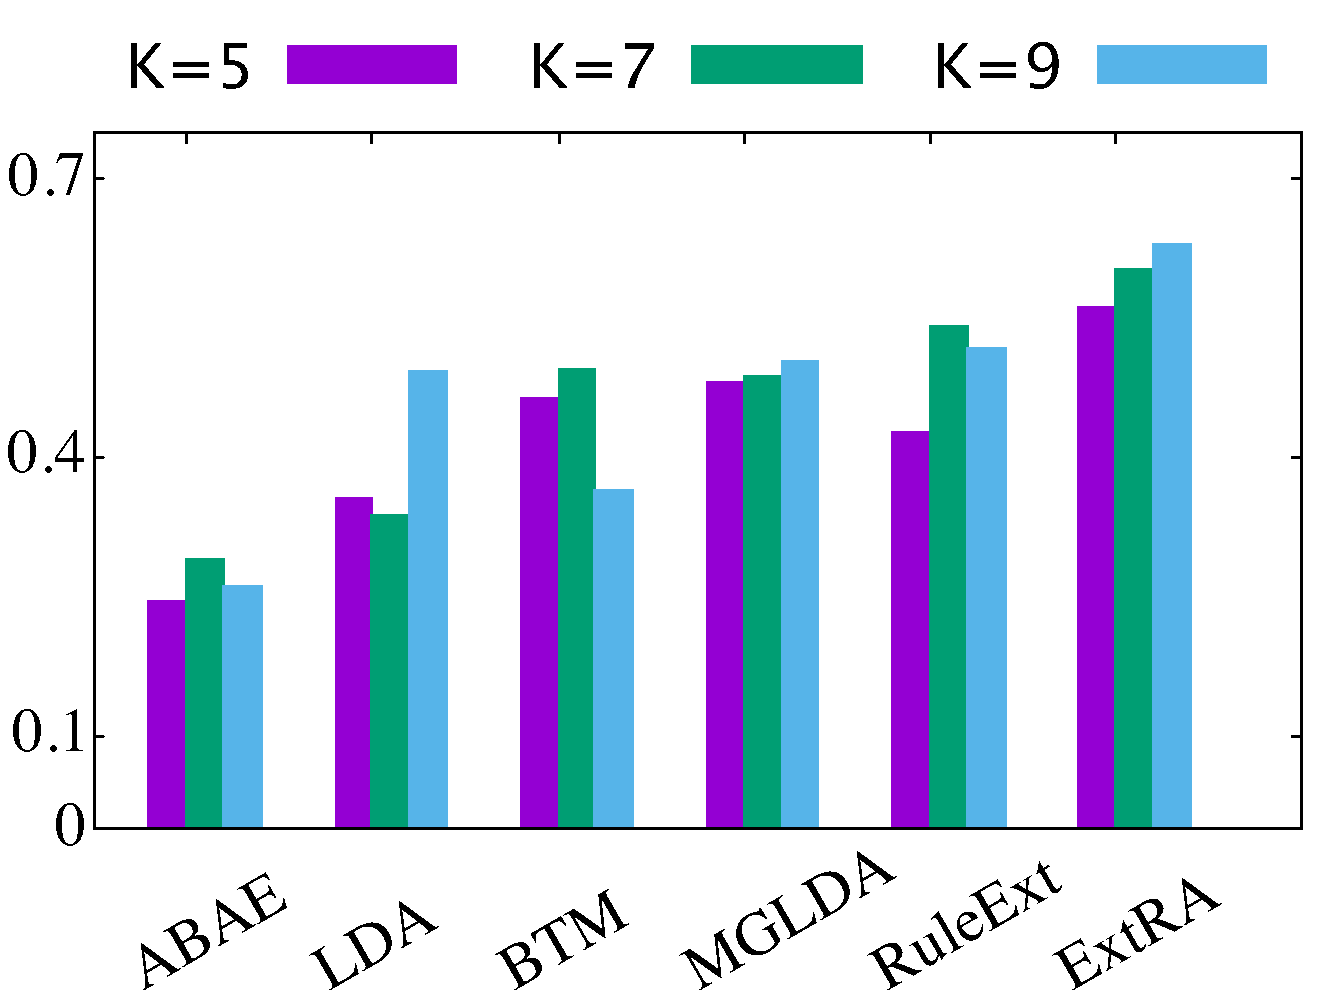
\includegraphics[width=\linewidth]{figures/laptop_s}
		\caption{laptop}
		\label{fig:laptop_s}
	\end{subfigure}%
	\begin{subfigure}{.333\textwidth}
		\centering
		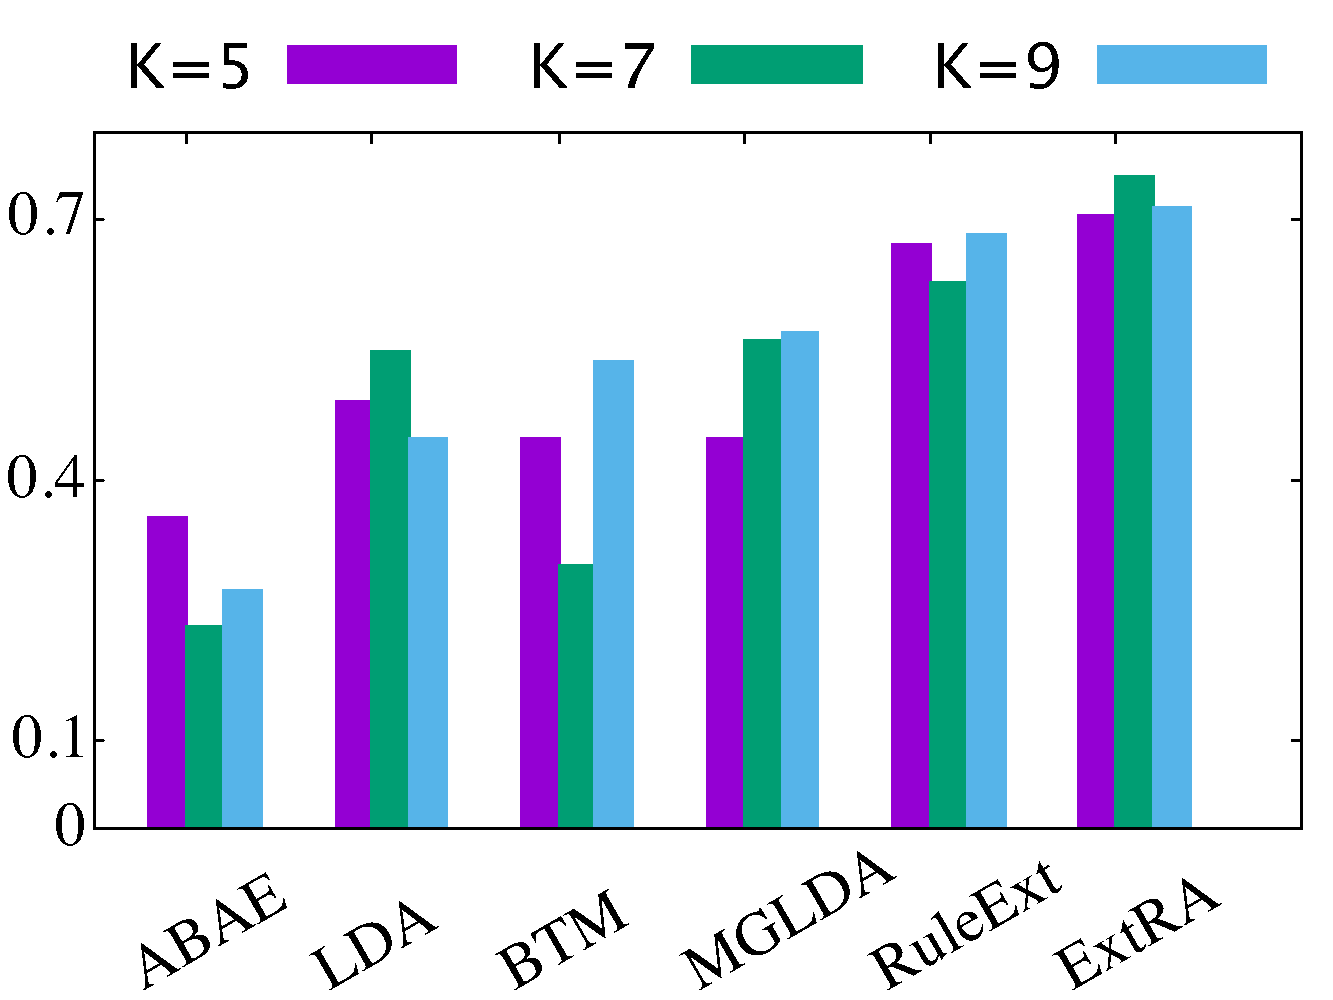
\includegraphics[width=0.99\linewidth]{figures/restaurant_s}
		\caption{restaurant}
		\label{fig:restaurant_s}
	\end{subfigure}
	
	\caption{Comparison of soft accuracies on all $K$s and categories }
	\label{fig:comparison_all_s}
\end{figure*}

To remedy this, we propose the \emph{soft accuracy}  evaluation measure.
We first align each generated aspect $a_k \in Aspects(m)$
with one golden aspect $l_j \in L^{(h)}$ (i.e. $align^{(h)}(a_k)=l_j$). 
We align the exact match terms together, and then choose the optimal alignment for the others by permuting all possible alignments. 
The optimal alignment $align^{(h)}(a_k)$ achieves
maximum soft accuracy.

Then we calculate the soft matching score between
$Aspects(m)$ and $L^{(h)}$ as 
$\sum_{k=1}^{K}sim(a_k, align^{(h)}(a_k))$,
where $sim$ is the cosine similarity computed by 
Glove~\cite{pennington2014glove}. 
We then compute the soft accuracy measure as follows:
%We sum such soft matching scores to represent the accuracy of the model. We then average such accuracies on 5 sets of labels from the 5 annotators as the soft accuracy measure:
\begin{equation}
sacc(m) =\frac{1}{H}\sum_{h=1}^{H}\sum_{k=1}^{K}sim(a_k, align^{(h)}(a_k)), 
\end{equation}
where $K$ could be $5$, $7$ and $9$
in the experiments.
We show the hard and soft accuracies
in \tabref{table:comparison} under the optimal $K$ for each category. 
The complete comparison results including $K=5,7,9$ for all categories are shown
in \figref{fig:comparison_all_h} (hard accuracy) and \figref{fig:comparison_all_s} (soft accuracy).
We can see that model ExtRA outperforms all the other baselines 
in all categories under both hard and soft accuracy measures.



%\begin{figure*}[th]
%	\subfigure[Similarity in Free version]{
%		\label{fig:simF}
%		\centering
%		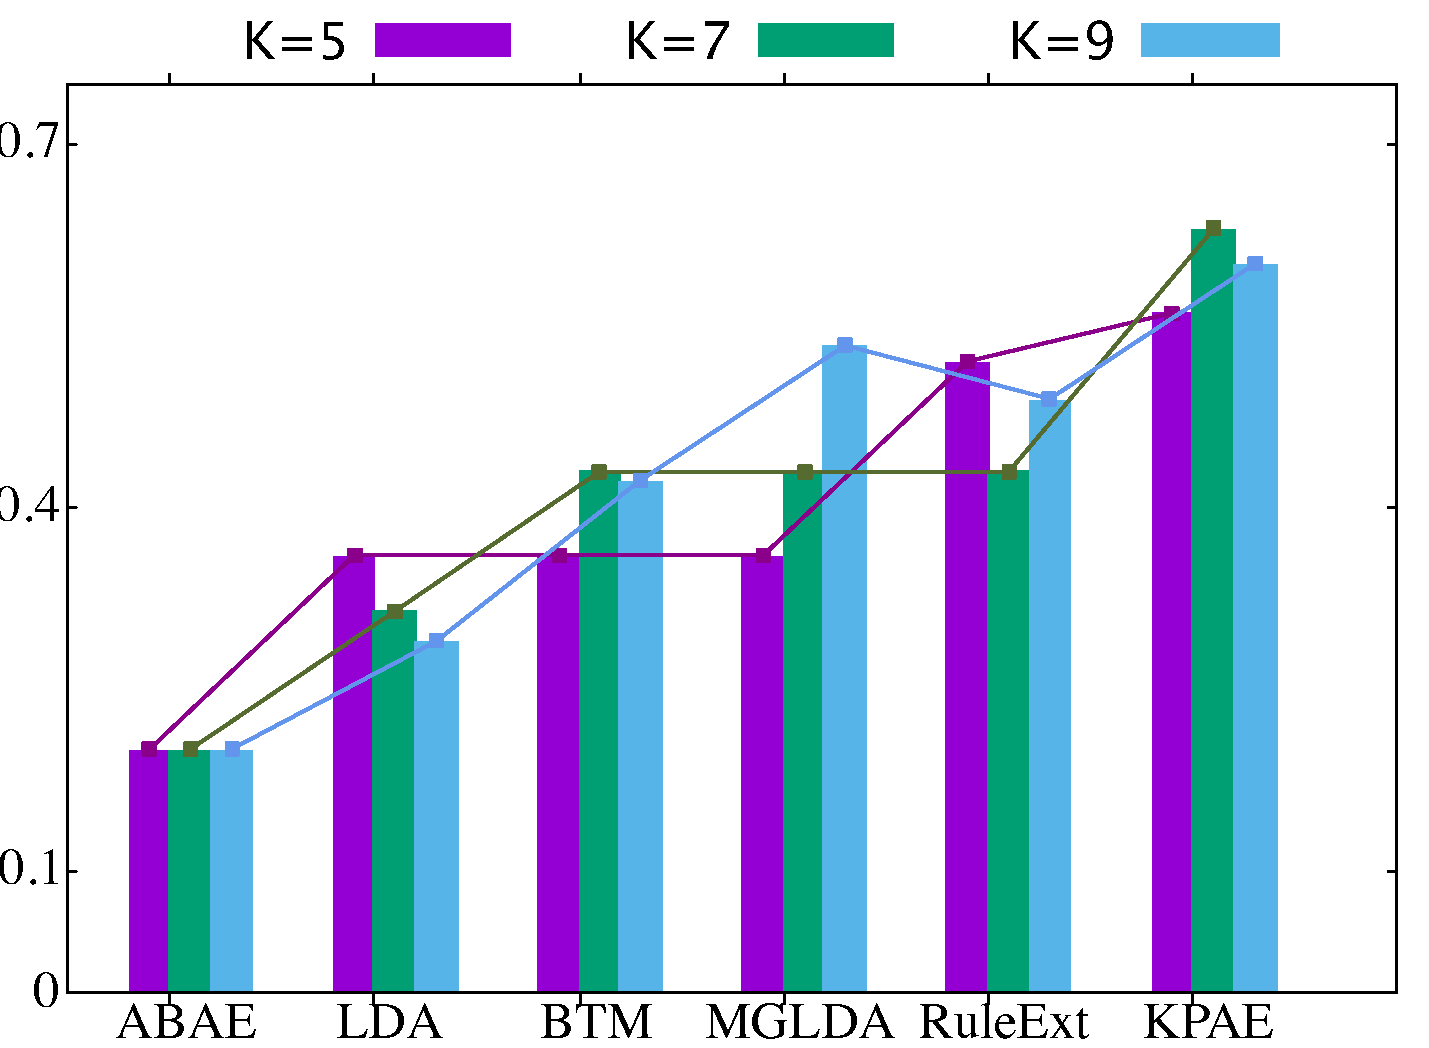
\includegraphics[width=2in]{figures/test}
%	}
%	\subfigure[Similarity in Trunc version]{
%		\label{fig:simT}
%		\centering
%		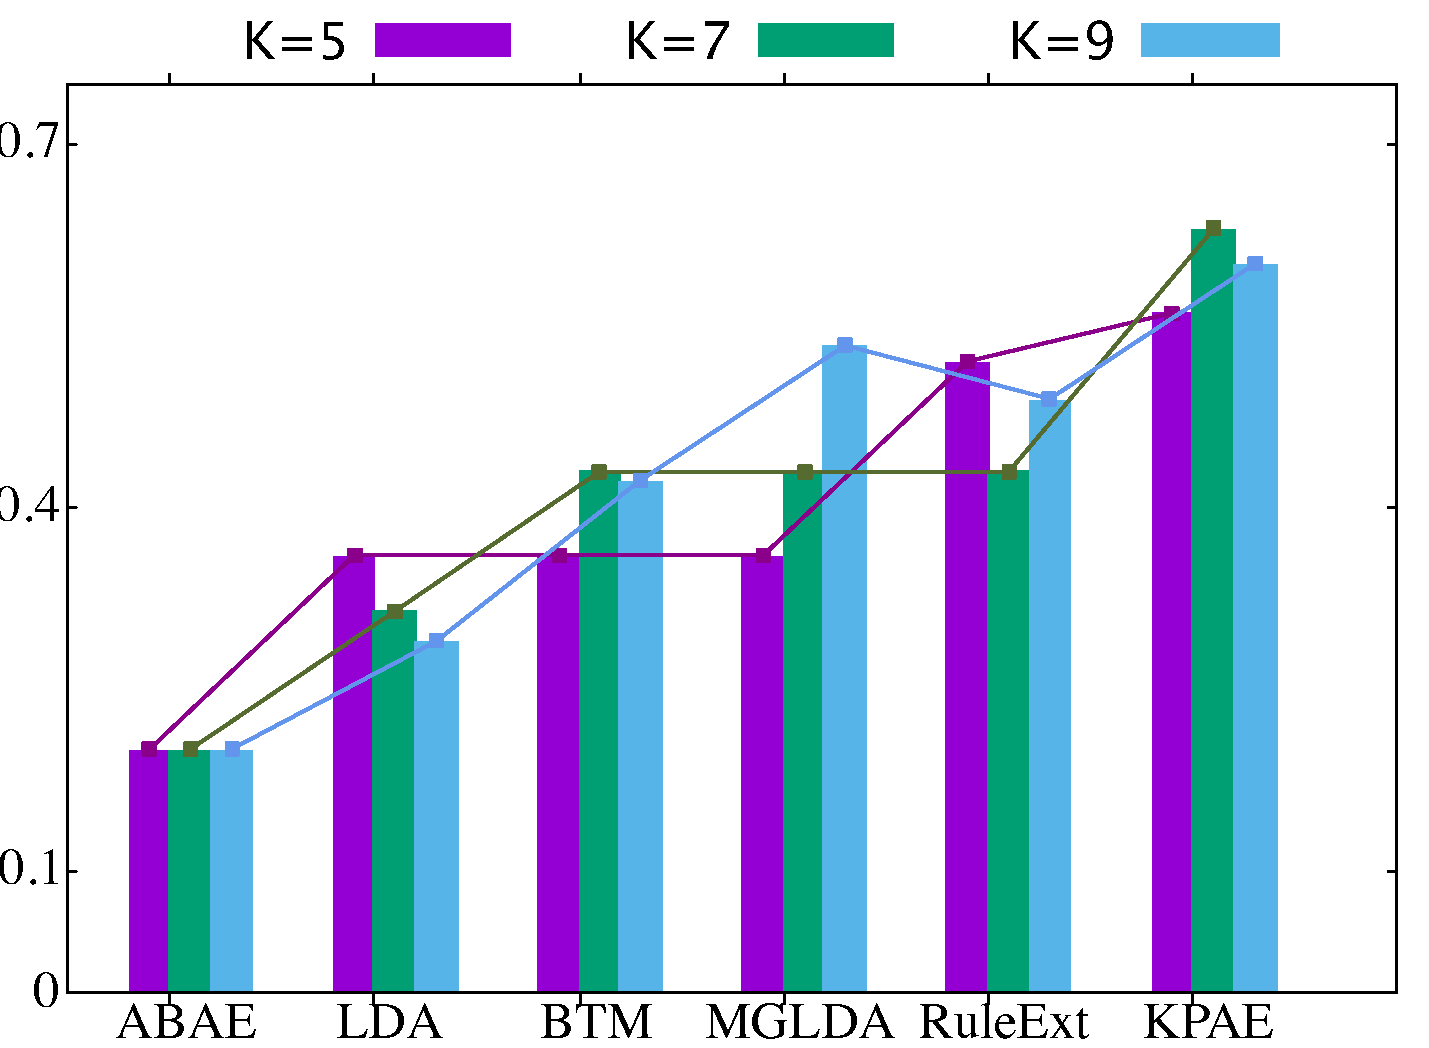
\includegraphics[width=2in]{figures/test}
%	}
%	\subfigure[Similarity in Exact version]{
%		\label{fig:simE}
%		\centering
%		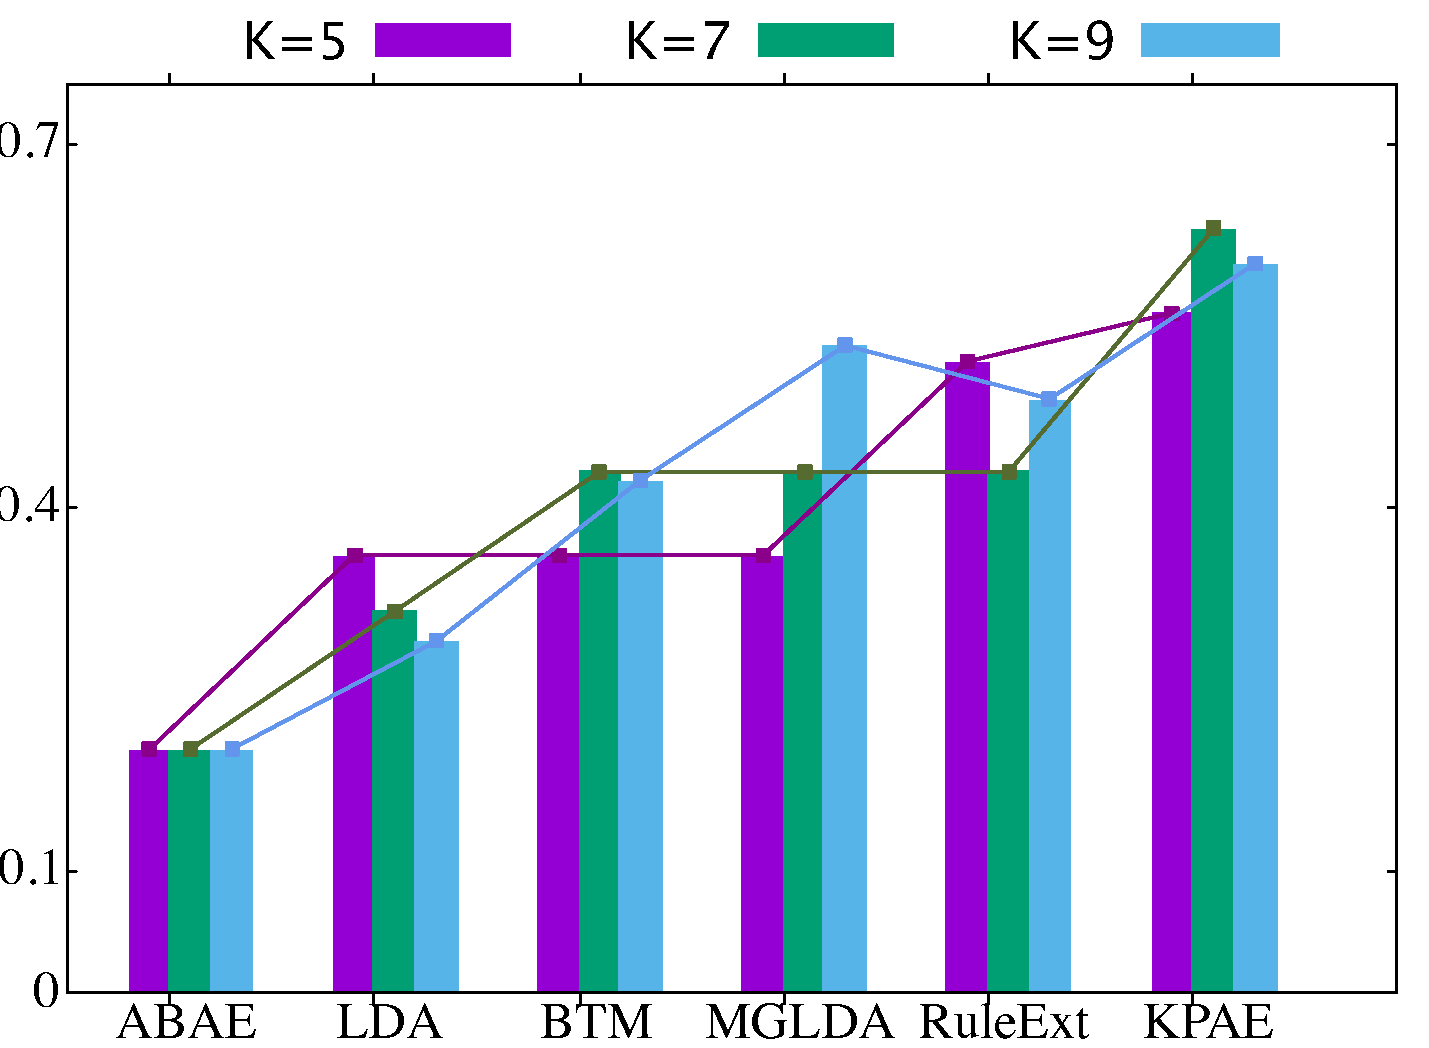
\includegraphics[width=2in]{figures/test}
%	}
%	\caption{Similarity of different length}
%	\label{fig:comparison_all}
%\end{figure*}

%\begin{figure*}[t!]
%\centering
%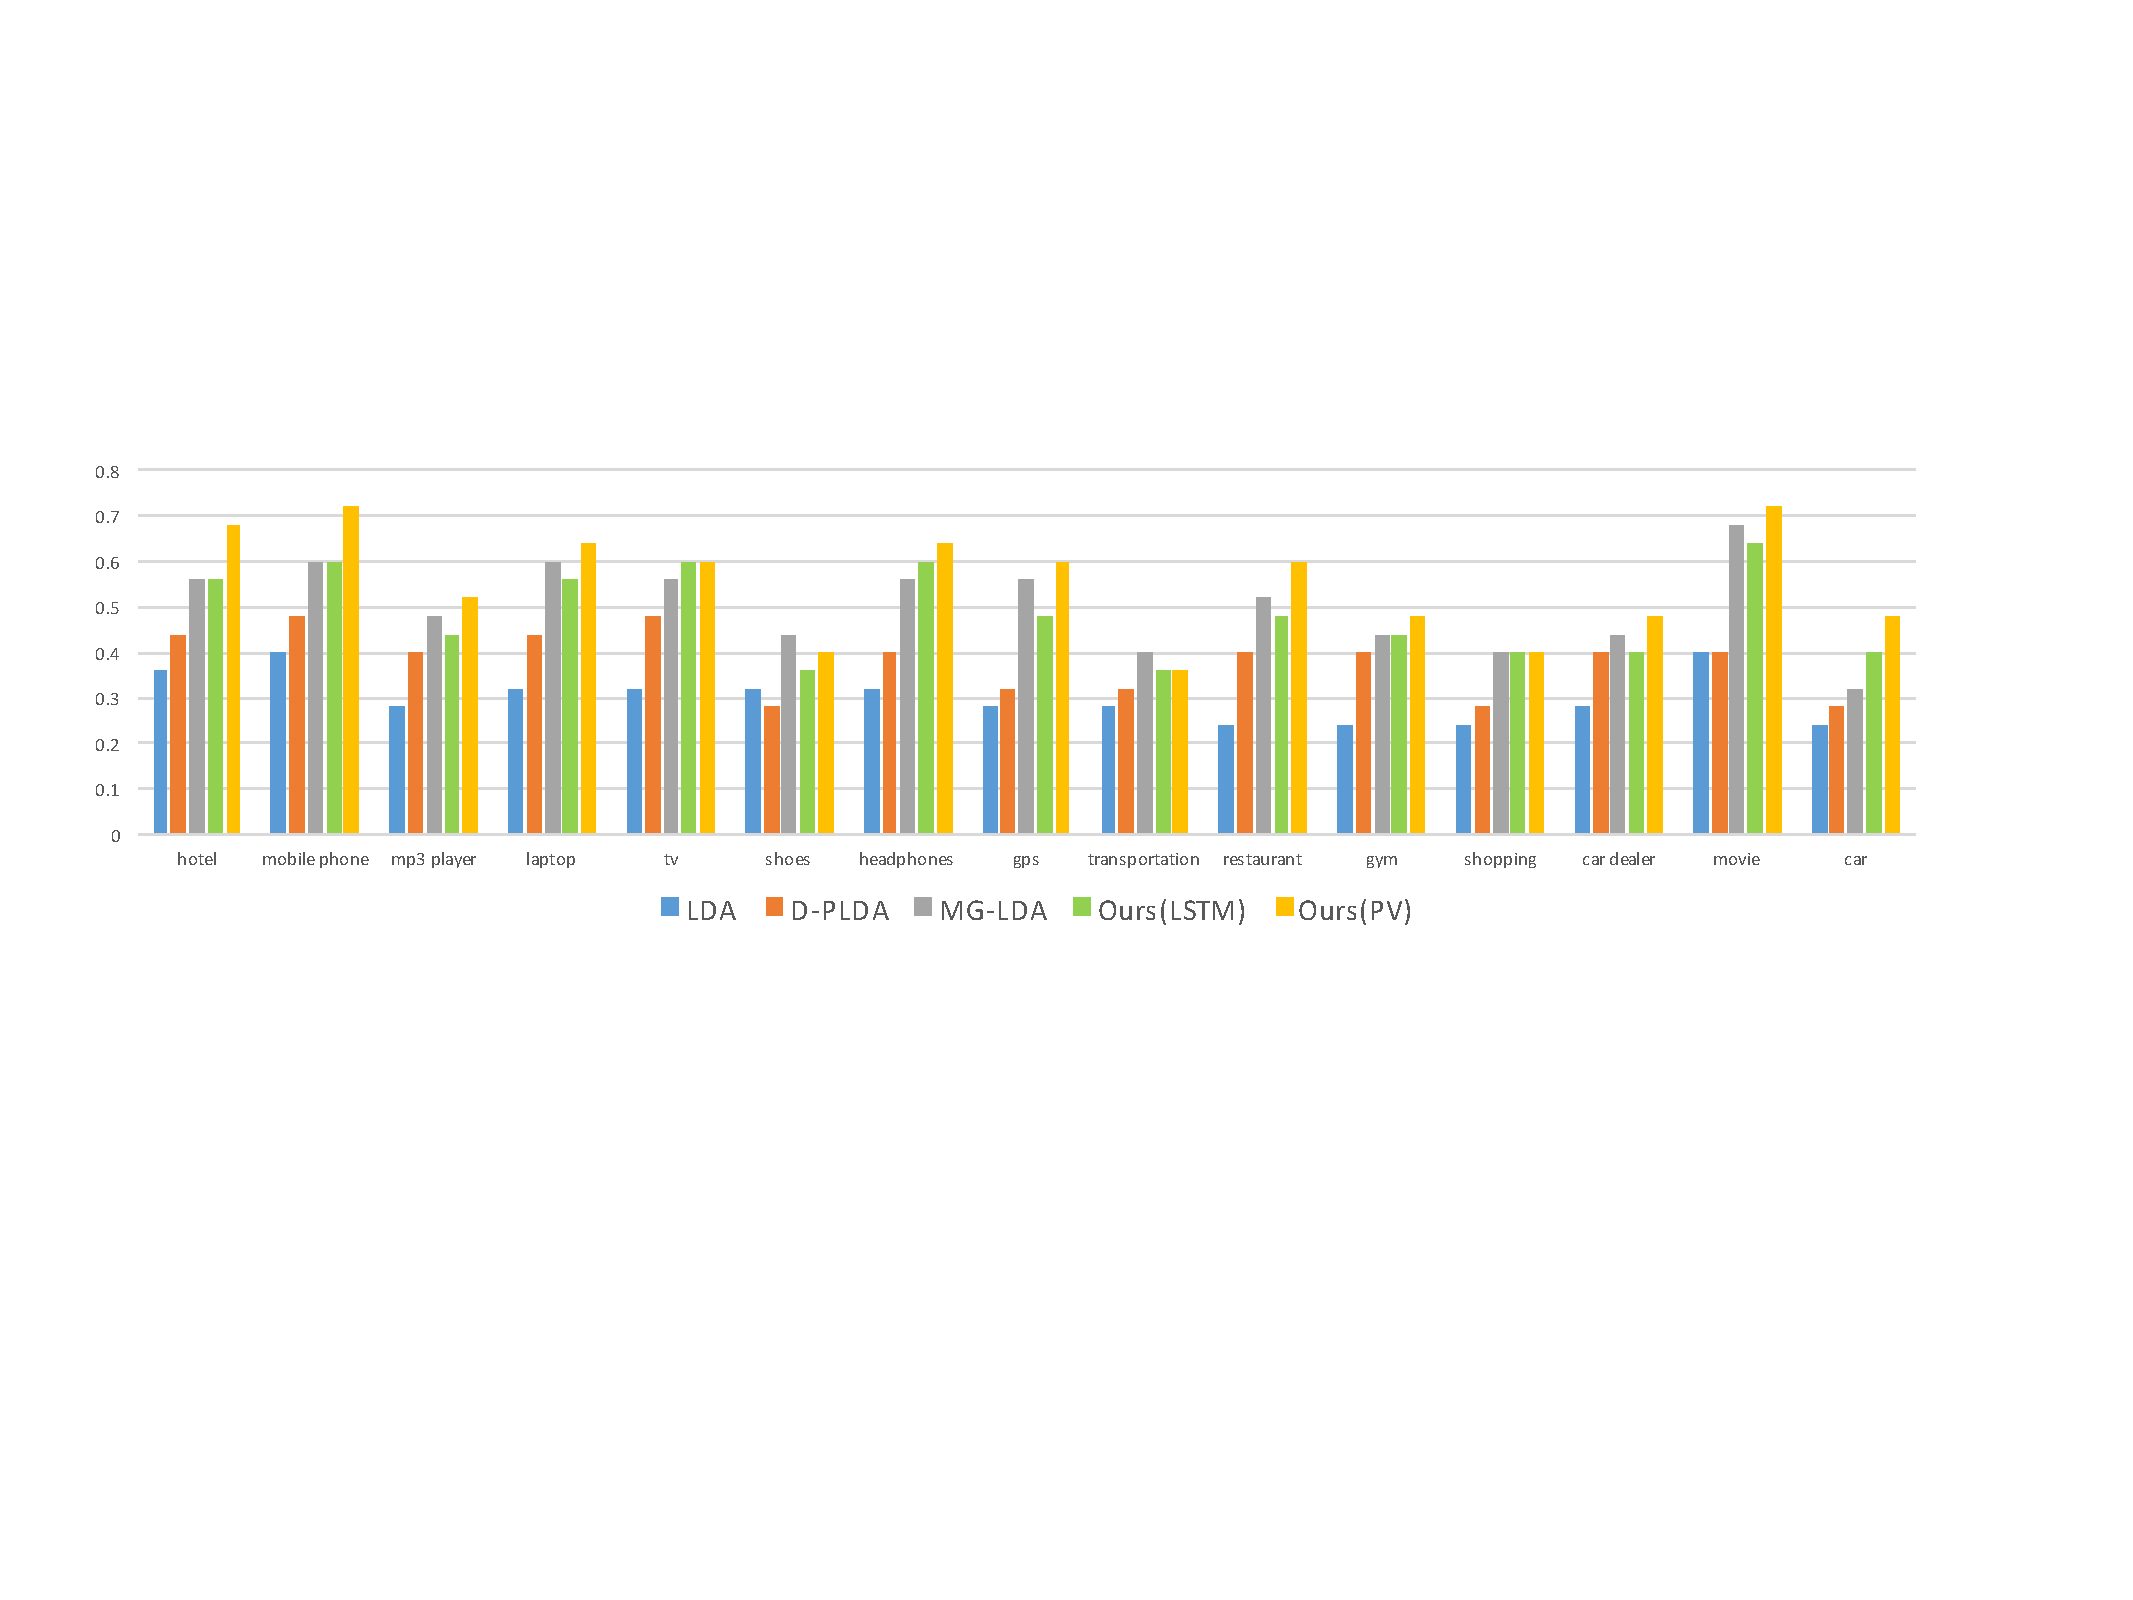
\includegraphics[width=2.0\columnwidth]{figures/results}
%\caption{Comparison of accuracies from different models on aspect extraction.}
%\label{fig:results}
%\end{figure*}  

%\ZY{Our approach alleviate the overlapping problem by using the aspect  taxonomy.}

%\subsubsection{Qualitative Analysis}
\subsubsection{Qualitative Analysis}

To qualitatively evaluate different models,
we present the extracted aspect terms
by each model with the number of optimal $K$
 from each domain in \tabref{table:aspect_words_a} and
 \tabref{table:aspect_words_b}. 
 
 
 \begin{table}[!th]
 	\small
 	\centering
 	\caption{Comparison of aspect clusters for PAE and ABAE on \textit{hotel}.}
 	\label{table:aspect_clusters}
 	\begin{tabular}{|c|l|}
 		\hline
 		\multirow{5}{*}{ABAE} & \textbf{room}, bathroom, bed, bedroom, miniscule, ensuite   \\
 		&  \textbf{accomodation}, solamar, donatello, stay   \\ 
 		&  repeatedly, shouted, apologised, \textbf{supervisor}, yelled   \\ 
 		&  excellent, great, terrific, awesome, \textbf{divine}, sensational  \\ 
 		&  alexanderplatz, loop, \textbf{tunnel}, block   \\  \cline{2-2}
 		\hline
 		\hline
 		\multirow{9}{*}{ExtRA} & \textbf{room}, dining room, dining experience   \\
 		&  \textbf{breakfast}, breakfast buffet, buffet \\ 
 		&  \textbf{staff}, reception staff, reception   \\ 
 		&  \textbf{location}, place, side, position   \\ 
 		&  \textbf{price}, cost   \\  
 		&  \textbf{bed}, linen, furniture, chair, furnishings, bed size \\
 		&  service, \textbf{internet}, internet access, shuttle service \\
 		&  \textbf{bathroom}, shower, tub, bath \\
 		&  \textbf{pool}, pool area, amenity, facility, swimming pool \\ \cline{2-2}
 		\hline
 	\end{tabular}
 \end{table}

Our model (ExtRA) has significant advantage over other baselines for that we can do better aspect extraction with reasonable results, and extract not only words but also phrases as prominent aspects, \textit{e.g. battery life}. 
The proposed model avoid the overlapping aspects appeared in our strong baseline 
(RuleExt) by implicitly deduplication using our grouping algorithm. 
For example, both \textit{picture} and \textit{photo} are extracted as top aspects in
the \textit{cameras} category, 
but they mean nearly the same concept. 
In addition, ExtRA generate each prominent aspect associated with
a group of supporting terms, expressing the prominent aspect in different ways
while traditional baselines can only extract the prominent aspects.
Among the baselines, only ABAE could infer such aspect clusters.
We further show the effectiveness of ExtRA by comparing
aspect clusters with ABAE in \tabref{table:aspect_clusters}.
For simplicity, we show the top terms in each aspect cluster on \textit{hotel}.
Each line in \figref{table:aspect_clusters} represents an aspect cluster, and
we highlight the extracted prominent aspect from ExtRA with bold font.
We can see that ABAE tends to cluster adjectives and verbs together
which is not suitable for the prominent aspect extraction task.

\begin{table}[!th]
	\small
	\centering
	\caption{The prominent aspect terms for \textit{hotel}, \textit{mp3} and \textit{cameras} }
	\label{table:aspect_words_a}
	\begin{tabular}{|c|c|p{0.6\columnwidth}|}
		\hline
		\multirow{6}{*}{\begin{tabular}{cc}
				hotel\\($K=5$)
		\end{tabular}} & LDA    & room, breakfast, location, pool, staff   \\ \cline{2-3}  
		%	& room, breakfast, location, pool, staff                            \\ \cline{2-3} 
		& BTM     & room, pool, location, staff, time                       \\ \cline{2-3} 
		& MGLDA   & room, breakfast, location, night, staff                      \\ \cline{2-3} 
		&  ABAE      & room, accommodation, supervisor, divine, tunnel \\ \cline{2-3} 
		& RuleExt & room, staff, hotel, location, bed                     \\ \cline{2-3} 
		& \textbf{ExtRA}   & \textbf{ room, breakfast, staff, location, price}                \\ \hline
		\multirow{11}{*}{\begin{tabular}{cc}
				mp3\\($K=9$)
		\end{tabular}}      &  \multirow{2}{*}{LDA}       & battery, button, work, player, music, video, ipod, quality, software                        \\ \cline{2-3} 
		& \multirow{2}{*}{BTM}     & battery, player, ipod, para, screen, work, music, software, headphone                      \\ \cline{2-3} 
		&  \multirow{2}{*}{MGLDA}     & song, battery, ipod, player, computer, quality, button, software, size                      \\ \cline{2-3} 
		& \multirow{2}{*}{ABAE}    & album, tone, middle, dollar, application, birthday, lightweight, buyer, holder        \\ \cline{2-3} 
		&  \multirow{2}{*}{RuleExt}   & quality, sound, player, drive, screen, feature, \mbox{battery, price, software}                 \\ \cline{2-3} 
		&  \multirow{2}{*}{\textbf{ExtRA}}      & \textbf{quality, sound, screen, control, display, \mbox{headphone, battery life, price, software}}      \\ \hline
		\multirow{11}{*}{\begin{tabular}{cc}
				cameras\\($K=9$)
		\end{tabular}}      & \multirow{2}{*}{LDA}     & lens, battery, screen, canon, water, video, mode, problem, quality                        \\ \cline{2-3} 
		& \multirow{2}{*}{BTM}     & para, battery, light, canon, lens, video, mode, quality, card                 \\ \cline{2-3} 
		& \multirow{2}{*}{MGLDA}   & lens, manual, battery, light, canon, pocket, mode, year, quality                  \\ \cline{2-3} 
		& \multirow{2}{*}{ABAE}    & portability, battery, photo, vacation, illinois, lens, mode, device, promotion        \\ \cline{2-3} 
		& \multirow{2}{*}{RuleExt} & camera, \textit{picture, photo}, quality, feature, shot, price, image, zoom                \\ \cline{2-3} 
		& \multirow{2}{*}{\textbf{ExtRA} }   & \textbf{picture, zoom, lens, control, speed, price, \mbox{battery life}, accessory, screen}       \\ \hline
	\end{tabular}
\end{table}

\begin{table}[!th]
	\small
	\centering
	\caption{The prominent aspect terms for \textit{mobile phone}, \textit{laptop} and \textit{restaurant} }
	\label{table:aspect_words_b}
	\begin{tabular}{|c|c|p{0.6\columnwidth}|}
		\hline
				\multirow{11}{*}{\begin{tabular}{ccc}
						mobile\\phone\\($K=9$)
				\end{tabular}}
%			{\begin{tabular}[c]{@{}l@{}}mobile phone\\($K=9$)\end{tabular}}
			     &    \multirow{2}{*}{LDA}   & service, battery, screen, work, music, blackberry, android, price, button                         \\ \cline{2-3} 
		&    \multirow{2}{*}{BTM}      & para, battery, screen, work, video, android, card, price, time                         \\ \cline{2-3} 
		&     \multirow{2}{*}{MGLDA}    & battery, quality, screen, work, android, venezuela, card, text, price                      \\ \cline{2-3} 
		&     \multirow{2}{*}{ABAE}    & flat, descent, kernel, bookmark, month, flagship, shutdown, representation, dealer        \\ \cline{2-3} 
		&    \multirow{2}{*}{RuleExt}      & phone, screen, camera, battery, price, quality, \mbox{feature, picture, app}                \\ \cline{2-3} 
		&    \multirow{2}{*}{\textbf{ExtRA}}    & \textbf{camera, quality, price, screen, battery life, \mbox{accessory, speed, keyboard, reception}}          \\ \hline
		\multirow{11}{*}{\begin{tabular}{cc}
				laptop\\($K=9$)
		\end{tabular}}   &    \multirow{2}{*}{LDA}     & google, apple, windows, screen, price, battery, game, problem, processor                   \\ \cline{2-3} 
		&    \multirow{2}{*}{BTM}   & google, apple, windows, screen, game, video, \mbox{problem, port, battery}                    \\ \cline{2-3} 
		&    \multirow{2}{*}{MGLDA}  & windows, screen, work, battery, speaker, keyboard, price, key, software                   \\ \cline{2-3} 
		&    \multirow{2}{*}{ABAE}    & bridge, cable, twitter, bezel, window, shutdown, opinion, holiday, explanation      \\ \cline{2-3} 
		&     \multirow{2}{*}{RuleExt} & laptop, computer, drive, screen, keyboard, \mbox{battery}, price, machine, feature              \\ \cline{2-3} 
		&   \multirow{2}{*}{\textbf{ExtRA}}  & \textbf{screen, graphic, price, drive, processor, hardware, battery life, system, speed}               \\ \hline
		\multirow{7}{*}{\begin{tabular}{cc}
				restaurant\\($K=7$)
		\end{tabular}}      &    LDA     & bar, room, service, food, time, pizza, chicken                     \\ \cline{2-3} 
		&  BTM       & room, food, time, les, das, chicken, work                      \\ \cline{2-3} 
		& MGLDA     & star, service, area, food, time, chicken, minute           \\ \cline{2-3} 
		& \multirow{2}{*}{ABAE}    & communication, killer, eatery, wright, chickpea, fireplace, tomorrow          \\ \cline{2-3} 
		& RuleExt    &  food, service, place, staff, price, experience, time              \\ \cline{2-3} 
		&  \multirow{2}{*}{\textbf{ExtRA}}  & \textbf{service, food, staff, flavor, atmosphere, \mbox{selection}, location}            \\ \hline
	\end{tabular}
\end{table}

\section{Implications}


\label{sec:implication}
Our main aim in this study was to address the problem of prominent aspect extraction, which benefits a multitude of downstream applications
such as aspect-based review summarization.
The existing methods mainly focus on 
fine-grained aspect extraction, which cannot adapt to 
the problem well.

We propose the ExtRA, an unsupervised
and effective system, for generating aspect clusters
as well as extracting prominent aspects from product reviews.
In \secref{sec:experiments}, 
we demonstrate the effectiveness of 
the components integrated within ExtRA.
The key insight of extracting prominent aspects
is that we value the aspect terms according to
the popularity (or coverage) and the semantic overlaps with each other.
We instantiate the popularity based on the data-driven approach of 
aspect extraction
and utilize the knowledge sources to facilitate 
the specification of semantic overlaps between aspects.
We further demonstrate the usefulness of the proposing strategies
and especially that the relation weighting scheme, which is the point for
the segmentation of aspect space, values the strength of 
subsumption relation between aspects based on the 
typicality score computed using Probase.






